\PassOptionsToPackage{full}{textcomp}
\documentclass[]{tufte-handout}
%\usepackage{fontspec}

% load babel package and options here
%\usepackage[p,osf]{ETbb} % osf in text, tabular lining figures in math
\usepackage{ETbb} % osf in text, tabular lining figures in math
\usepackage[scaled=.95,type1]{cabin} % sans serif in style of Gill Sans
\usepackage[varqu,varl]{zi4}% inconsolata typewriter
\usepackage[T1]{fontenc} % LY1 also works
\usepackage[libertine,vvarbb]{newtxmath}
%\usepackage[cal=boondoxo,bb=boondox,frak=boondox]{mathalfa}

%\geometry{showframe} % display margins for debugging page layout

\usepackage{graphicx} % allow embedded images
%  \setkeys{Gin}{width=\linewidth,totalheight=\textheight,keepaspectratio}
  \graphicspath{{graphics/}} % set of paths to search for images
\usepackage{amsmath}  % extended mathematics
\usepackage{booktabs} % book-quality tables
%\usepackage{units}    % non-stacked fractions and better unit spacing
\usepackage{multicol} % multiple column layout facilities
\usepackage{lipsum}   % filler text
\usepackage{fancyvrb} % extended verbatim environments
  \fvset{fontsize=\normalsize}% default font size for fancy-verbatim environments
\usepackage{gensymb} % provides symbols like \degree
\usepackage{ragged2e} % enables hyphenation in ragged-right justification
\usepackage[normalize-symbols]{textalpha} %enables \textalpha for alpha symbol etc.

\usepackage{hyperref} % enables styling of href and url
\hypersetup{
    pdftitle={Mechanisms},
    pdfauthor={Barry Linkletter},
    colorlinks=true,
    linkcolor=blue,
    filecolor=magenta,      
    urlcolor=blue,
    pdfborder={0 0 0},
    frenchlinks=false,
    pdfpagemode=FullScreen,
    }
    \urlstyle{same}
\makeatletter
% Inspired by http://anti.teamidiot.de/nei/2009/09/latex_url_slash_spacingkerning/
% but slightly less kern and shorter underscore
\let\UrlSpecialsOld\UrlSpecials
\def\UrlSpecials{\UrlSpecialsOld\do\/{\Url@slash}\do\_{\Url@underscore}}%
\def\Url@slash{\@ifnextchar/{\kern-.03em\mathchar47\kern-.15em}%
    {\kern-.0em\mathchar47\kern-.08em\penalty\UrlBigBreakPenalty}}
\def\Url@underscore{\nfss@text{\leavevmode \kern.06em\vbox{\hrule\@width.3em}}}
\makeatother

\usepackage{enumitem} % allows resuming enumerate lists.
\usepackage{mathtools}
\usepackage{mhchem}

\usepackage{siunitx}
    \sisetup{
        uncertainty-mode        = separate,
        tight-spacing           = true}

\usepackage{nicefrac}

\usepackage[nospace]{varioref}
    \renewcommand\reftextfaceafter{on the following page}
    \renewcommand\reftextafter {on the next page}
    \renewcommand\reftextfacebefore{on the previous page}
    \renewcommand\reftextbefore {on the previous page}

\newcommand{\tss}[1]{\textsuperscript{#1}}

\usepackage[english]{babel}
\usepackage{float}
\usepackage{stackrel}

\usepackage[shortconst]{physconst}

\usepackage[normalem]{ulem}  % provides strikethrough \sout{}

\usepackage{newfloat}
\DeclareFloatingEnvironment[
  fileext = los ,
  listname = {List of Schemes} ,
  name = Scheme
]{scheme}

\usepackage{newfloat}
\DeclareFloatingEnvironment[
  fileext = loe ,
  listname = {List of Eqs} ,
  name = Equation
]{equate}

\usepackage{listings}
\usepackage{longtable}
\usepackage{tabularx}

%%%%%%%%%%%%%%%%%%%%%%%%%%%%%%%%%%%%%%%%%%%%%%%%%%%%%%%%%%%

\title{Literature Values for $\rho$, $a_{_{\ce{H2O}}}$ \& $H_0$}
\author[Barry Linkletter]{Barry Linkletter}
\date{} % without \date command, current date is supplied


\begin{document}

\justifying

\maketitle
\marginnote[-15mm]{This document was produced using the \LaTeX\ typesetting language with the Tufte-handout document class. Chemical diagrams were created in \textit{ChemDoodle} and calculations and plotting were performed using \textit{Python} tools in a \textit{Jupyter Notebook}. Diagrams and plots were further edited in \textit{Affinity Designer}\vspace{3mm}}
%\justify
\begin{abstract}

\noindent This is an update to the interpolation exploration that I have previously presented. Here I will use more recent data sets for $a_{\ce{H2O}}$ and $H_0$ vs. concentration of \ce{H2SO4} (expressed in molality, molarity and \% mass). I will use polynomial fits and create parameterized models to convert between the data sets. This will be more portable than the interpolator functions used previously.\sidenote[][-6mm]{\textsc{Warning}: After 19 pages of work, I concluded that interpolation works best in most cases for these data sets. Skip to the end and read the rest if you want to learn more about polynomial modelling in \textit{Python}.}

\end{abstract}




\section{Introduction}

In a previous exploration document, I presented methods for interpolating tables of data for values of $H_0$, $a_{\ce{H2O}}$ and density of mixtures of water and sulphuric acid.\sidenote[][-10mm]{See ``Interpolating Literature Data Sets'', available via our Moodle site.} Using data tables from the literature, a smoothing interpolation function was applied to create an interpolation function that would return a value when given a concentration of a \ce{H2SO4}/\ce{H2O} mixture. These interpolator functions, provided from the \texttt{scipy.interpolate} library, tracked very closely to the experimental data but tended to deviate at the extremes of the data sets. These deviations were small but became a problem when the interpolated values were also tiny. I ran into an issue where the interpolation for $a_{\ce{H2O}}$ in very concentrated sulphuric acid mixtures was returning negative values. If I want to use data at greater than \qty{99}{\percent} \ce{H2SO4}, I will need a better system for extracting data from these data tables.

Also, the interpolator functions generated by the \texttt{scipy.interpolate} library are a black box, and cannot be expressed in printed form. Having the code available via an interactive \textit{Python} notebook does allow the reader to access exactly what was done,\sidenote[][-60mm]{The \textit{Python} notebook for the previous interpolation exploration can accessed via Google Colab at \url{https://colab.research.google.com/github/blinkletter/4410PythonNotebooks/blob/main/Class_30/Yates-interpolators.ipynb}. If you have internet access, you can investigate the code and reproduce my results easily. But, when the end of civilization comes to pass, those who seek to follow in my footsteps will only have these printed words found on singed paper in the rubble. That is why I want to build these parameterized models.\vspace{2mm}} but I find it more satisfying when the methodology can be expressed in writing.

The data that I had used to build the interpolator functions for $a_{\ce{H2O}}$ was from a data set reported by Giauque in 1960.\sidenote[][-20mm]{``The Thermodynamic Properties of Aqueous Sulfuric Acid Solutions and Hydrates from 15 to \qty{300}{K}.'' W.F. Giauque, E. W. Hornung, J. E. Kunzler, T. R. Rubin., \textit{J. Am. Chem. Soc.}, \textbf{1960}, \textit{82}, 62-70. \url{https://doi.org/10.1021/ja01486a014} \vspace{1mm}\label{ref:giauque}} I also had access to a data set produced by Rard in 1976.\sidenote[][0mm]{``A review of the osmotic coefficients of aqueous sulfuric acid at \qty{25}{\degreeCelsius}'' J.A. Rard, A. Habenschuss, F.H. Spedding,  \textit{J. Chem. Engin. Data}, \textbf{1976}, \textit{21}, 374-379. \url{https://doi.org/10.1021/je60070a002} \vspace{1mm}\label{ref:rard}} I have since come to realize that these data sets are based on polynomial fits of previous literature data. Over the years other groups have measured $a_{\ce{H2O}}$ using a variety of methods and this data has been used in similar models based on polynomial fits.\sidenote[][0mm]{``Activity and osmotic coefficients of aqueous sulfuric acid at 298.15 K.'' Bert R. Staples, \textit{J. Phys. Chem. Ref. Data,} \textbf{1981}, \textit{10}, 779–798. \url{https://doi.org/10.1063/1.555648}\vspace{1mm}\label{ref:staples}}


I will be using polynomial fits to create parameterized models that predict $a_{\ce{H2O}}$ in units of apparent mole fraction and apparent molar concentration from concentration data reported in units of \%mass. I will compare my results with those presented by Cox, who seems to have performed a similar exercise.\sidenote[][-3mm]{``Excess acidities.'' Robin A. Cox,  \textit{Adv. Phys. Org. Chem.}, \textbf{2000}, \textit{35}, 1-66. \url{https://doi.org/10.1016/S0065-3160(00)35011-0}\vspace{1mm}\label{ref:cox}}

\clearpage
\section{The Plan}

In my own exploration\sidenote[][0mm]{See ``Extreme Ester Hydrolysis'', available via our Moodle site.\vspace{2mm}} of the results reported by Yates and McClelland for ester hydrolysis\sidenote[][-0mm]
{``Mechanisms of ester hydrolysis in aqueous sulfuric acids.''
K. Yates, R.A. McClelland,
\textit{J. Am. Chem. Soc.}, \textbf{1967}, \textit{89}, 2686-2692.
\url{https://doi.org/10.1021/ja00987a033}\vspace{1mm}\label{ref:ref1}}
in concentrated sulphuric acid, I chose to express the value for $a_{\ce{H2O}}$ in terms of effective molar concentration rather than mole fraction. The tables of Giauque\tss{\ref{ref:giauque}}, Rard\tss{\ref{ref:rard}} and Staples\tss{\ref{ref:staples}} all report values for $a_{\ce{H2O}}$ in terms effective mole fraction of water versus the concentration of \ce{H2SO4} expressed as molality. However, the data tables that I have for $H_0$ use \%mass of \ce{H2SO4}. I need a model that will give me a value for $a_{\ce{H2O}}$ when given \%\ce{H2SO4}. With this tool, I can have values for both $a_{\ce{H2O}}$ and $H_0$ at any given value of \%\ce{H2SO4}. 

The CRC 	ook\sidenote[][-0mm]{CRC Handbook of Chemistry and Physics, 106\textsuperscript{th} ed. \textbf{2025}, J.R. Rumble, ed., \textit{CRC Press, Taylor \& Francis, Boca Raton, FL}. \url{https://library.upei.ca/chem} or get the \href{https://hbcp-chemnetbase-com.proxy.library.upei.ca/documents/05_29/05_29_0081.xhtml?dswid=9598}{PDF  here} or \href{https://hbcp-chemnetbase-com.proxy.library.upei.ca/contents/ArchiveSearch.xhtml?dswid=9598\&faces-redirect=true\#}{here}.\vspace{2mm}\label{ref:crc}}
provides this very information in data tables for the density of sulphuric acid mixtures. I hope to demonstrate that I can reach the same results.  Below is my plan for building the parameterized polynomial models\ldots.  

%
\begin{enumerate}

\item I will convert the molal concentrations reported in the data sets of Giauque, Rard and Staples to \%\ce{H2SO4} and molar concentrations. I will compare my results to those in the data tables of the CRC Handbook to increase my personal confidence that I did this correctly. 

\item I will also establish my models for converting molal to \%\ce{H2SO4} and compare them to literature models. I will create a data set for converting molar concentration ($M$) to \%\ce{H2SO4} ($w$) and vice-versa. Molality ($m$) can be concerted to $w$ by math. To convert $M$ we will need the measured density included in the calculation. 

\item I will build a model for $a_{H_2O}$ using the data sets of Giauque, Rard and Staples and fit the data to a polynomial\sidenote[][0mm]{All three of these data tables are, in fact, the output of parameterized models that are based on extensive data obtained by the authors or from literature. I am reverse-engineering models for which I have the outputs, but not the parameters.\vspace{2mm}} using \%\ce{H2SO4}. I will compare the data. If there is no major disagreement, I will combine the data sets and make a model. I will also compare my model to literature models for $a_{H_2O}$.\sidenote[][0mm]{Zhang et al. have recently presented a complex parameterized model for predicting the value of $a_{\ce{H2O}}$ in terms of mole fraction from the calculated mole fraction of the mixture. See ``An accurate water activity model for sulfuric acid solutions and its implementation on moisture sorption isotherm determination.'' L. Zhang, P.M. Grace,  D.-W. Sun, \textit{Drying Technology}, \textbf{2022}, \textit{40}, 2540-2549. \url{https://doi.org/10.1080/07373937.2020.1869037}.\vspace{2mm}} 

\item I will combine the acidity function data sets of Gillespie \& Peel, Johnson, and Jorgenson and fit this to a polynomial model. I will produce a parameterized model that represents the data table and predicts the value of $H_0$ from \%\ce{H2SO4}. I will not use the data set of Tickle, which differs significantly from the above, or the data set of Paul \& Long, which is very different at high acidities. I think that I will plot all five sets of data to show where they agree and diverge. 

\item I will convert the data from Cox\tss{\ref{ref:cox}} that is given in terms of molarity to \%mass. I will compare this to his second data set that is uses \%mass. This would be an attempt to confirm that our conversion method is working as well as the undocumented method that was used by Cox.\sidenote[][-10mm]{I am ``training'' a model using a data set and then validating that model against an independent data set. If all goes well, I can go forward with my model to predict a property from an input. This is how AI models work. They are all just models that predict and output when given an input. The whole world is currently fascinated by words produced from a very complex curve fit.} 

\end{enumerate}

 

%Here we go.

\section{1. Molality to Molarity and Percent}\label{sec:one}

Molal? Why not molar or percent weight? Molarity ($M$ or \unit{\mole\per\liter}) is a favourite of bench chemists. It related directly to rate constants and can be used as a measure of concentration in gas-phase chemistry, as long as the volume does not change. Volume changes in liquids are considered to be insignificant by most milquetoast room-temperature sea-level chemists.\sidenote[][0mm]{We salute the rocket scientists and chemical engineers that operate far beyond the borders of standard temperature and pressure. No one really needs all ten of their fingers.\vspace{2mm}} Molarity also takes a bit of fiddling. One must add so many moles of solute to a solution, mix until dissolved, and then carefully dilute to the final volume.

Molality ($m$ or \unit{\mole\per\kilo\gram}) is a measure of concentration that is independent of volume. It is a standard concentration in chemical engineering data sets because it will not change with temperature or pressure. It is also very easy to set molal concentration. One just throws a set amount of solute into a kilogram of water. Done. As a result, many data tables from the literature use units of molality ($m$) or percent weight ($w$),\sidenote[][0mm]{In this document the following abbreviations will be used: $M$ is molarity (moles in a total volume of one litre); $m$ is molality (moles added to a kilogram of solvent); $w$ is percent mass (mass solute/total mass); $\rho$ is density (\unit{{\gram\per\centi\meter\cubed}} or \unit{{\kilo\gram\per\meter\cubed}}). \vspace{2mm}} both of which are interconvertible by simple math.\sidenote[][0mm]{The following constants will be used: mole weight of \ce{H2O} is \qty{18.015}{\gram\per\mole}; mole weight of \ce{H2SO4} is \qty{98.079}{\gram\per\mole}.\vspace{2mm}}
\begin{align}
w &= \frac{m \cdot 98.079}{1000}100 \\
m &= \frac{\frac{w}{100}98.079}{\frac{w}{100}98.079 + \left(1-\frac{w}{100}\right)18.015}
\end{align}


Converting from molality to molarity is trivial, but one needs to know the density of the mixture.
\begin{equation}
M =  \frac{m\cdot \rho}{m \cdot 98.079 + 1000}
\end{equation}
Densities must be measured or found in data tables. A table that reports for densities of mixtures of sulphuric acid and water according to molal, molar and percent concentrations is available in the CRC Handbook.\tss{\ref{ref:crc}} I can use this table to check my math for interconverting the three concentration values and you can check my math by examining the \textit{Python} notebook that I have made available.\sidenote[][-0mm]{The \textit{Python} notebook for all following calculations and plots can accessed via Google Colab at \url{https://colab.research.google.com/github/blinkletter/4410PythonNotebooks/blob/main/Class_30_Yates_New/ParameterizedModels.ipynb}.\vspace{2mm}\label{ref:modelpython} }

I have used the molal concentrations ($m$) of \ce{H2SO4} to calculate values for percent mass ($w$) and molarity ($M$) using the density data table from the CRC handbook. I plotted the differences between my calculations and the reported values in that CRC table, and the results are identical within the precision of the numbers available. See Figure~\vref{fig:percentwmolarity} for these plots. My math agrees with the math of the editors of the CRC Handbook. More importantly, this exercise shows that there are no typographical errors in the four columns of data in that table.\sidenote[][0mm]{I typed these values or used sketchy OCR data from images of the written pages and the corrected the many errors. Transcribing data is a common source of error. Always validate your databases.} We have completed the first goal in our plan: we can convert between units of $m$, $M$, and $w$ within a data table for density.

\begin{figure}
  \centering
  \caption{Plots of differences between converted values for concentration and the corresponding reported values in the CRC data set. All differences are within the precision of the reported values: \\ a) Percent weight ($w$) from molality ($m$); \\ b) molarity ($M$) from molality ($m$). \\ $\longleftarrow$} 
 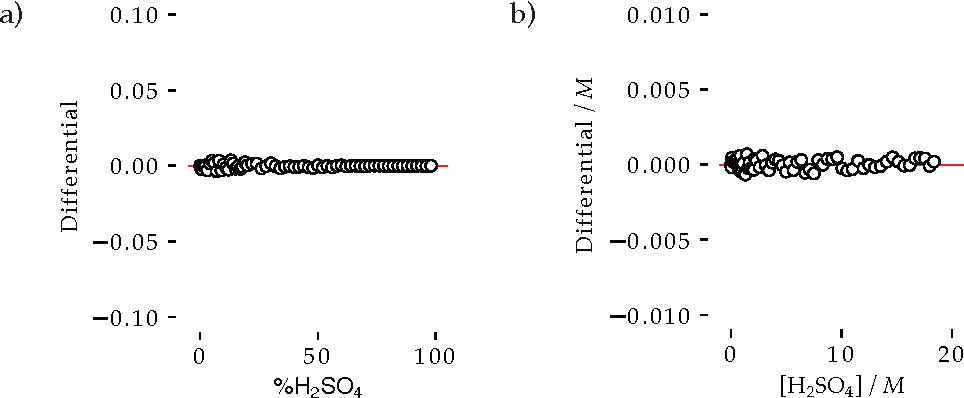
\includegraphics[scale=0.65]{images/differentials} 
  \label{fig:percentwmolarity}
\end{figure}


\newpage

\section{2. A Model for Density vs. $w$ }

The values of concentration in terms of molality or \unit{\percent\ce{H2SO4}} ($w$) are directly related to each other. However, conversion of these two units to molarity requires knowing the density of the given mixture, which is a measured value. We used the densities listed in the data tables for the exercise in section~1 above. But of we want a value for density at any value of $w$ or $m$, then we will need a model that predicts density vs. $w$. First we will need a reliable data set. Let us compare some data sets other than the one presented in the CRC handbook.

\subsection{Literature Density Data Sets}

A stated above, the density data for sulfuric acid-water mixtures at \qty{20}{\degreeCelsius} was obtained from the CRC Handbook. A second table available in the online-only edition of the CRC handbook also presents density data at a range of temperatures between \num{0} and \qty{100}{\degreeCelsius}.\tss{\ref{ref:crc}} This data appears in many works throughout the last century, such as Perry.\sidenote[][-6mm]{``Perry's Chemical Engineers' Handbook, 7\tss{th} ed.'' \textit{McGraw-Hill, New York}, \textbf{1997}, D.W. Green, J.O. Maloney, Eds., Available via interlibrary loan. See table 2-101 on page 2-107.\vspace{2mm}\label{ref:perry}} All of these data sets are clearly results of a parameterized model. These models are slight adjustments to a data set presented in 1905 by Bien \& Domke.\sidenote[][-0mm]{``Über Dichte und Ausdehnung der Schwefelsäure in wässeriger Lösung, ein Beitrag zu ihrem physikalisch-chemischen Verhalten.'' J. Domke, W. Bein, \textit{Z. Anorg. Chem.}, \textbf{1905}, \textit{43}, 125-181. \url{https://doi.org/10.1002/zaac.19050430114}. Available via interlibrary loan.\vspace{2mm}\label{ref:domke}} I did my best to translate the German text. It appears that the authors assembled sets of density data reported by many previous works dating back as far as 1861 and also measured their own data. They then fit this data to an undocumented parameterized model and produced a final table of densities at every integer percent weight between 1 and \qty{100}{\percent} at temperatures between \num{0} and \qty{60}{\degreeCelsius}. Their data was standardized to a density of pure water of \qty{1.0000}{\gram\per\centi\meter\cubed} at \qty{15}{\degreeCelsius}. The modern tables adjust for our current definition of the density of water, but otherwise use the data as presented in 1905. There are many reports in the literature of density data at various concentrations and temperatures. When I have examined them, I find that they usually agree to the fifth decimal point with the Domke data set.

That is a long way to say that the data set from the CRC handbook is the gold standard for today's chemist. Even though it is likely to be a polynomial fit of a data table from 1905 that was itself a polynomial fit of data\sidenote[][-10mm]{Or perhaps the data was carefully plotted on a large sheet of fine graph paper and then a French curve was used to create a best line through the data. That method is the essentially the same as modern bspline parameterized models made using a fancy computer.} from the 19\tss{th} century. Densities of liquids are easy to measure and it is no surprise that these values have been precisely known for hundreds of years.

\subsection {Our Data} 

First I will gather the data.  I have access to the following data sets\ldots

\begin{itemize}
\item 100 data pairs of $\rho$  at integer values of  $w$ (\num{0} to \qty{100}{\percent}) for temperatures in the range of \num{0} and \qty{100}{\degreeCelsius}. This data is from Perry\tss{\ref{ref:perry}} and is based on an undocumented parameterized model from Domke.\tss{\ref{ref:domke}} This model is also the basis for the CRC Handbook data tables.\tss{\ref{ref:crc}} 
\item 30 data pairs of measured values of $\rho$  and  $w$ (\num{0} to \qty{99.6}{\percent}) for the temperatures of \num{0}, \num{25}, \num{50} and \qty{75}{\degreeCelsius}.\sidenote[][0mm]{``The Viscosities of Mixtures of Sulfuric Acid and Water.'' F. H. Rhodes, C. B. Barbour, \textit{Ind. Eng. Chem.}, \textbf{1923}, \text{15}, 850-852. \url{https://doi.org/10.1021/ie50164a033}.\vspace{2mm}\label{ref:rhodes}}
\item 27 data pairs of measured values of $\rho$  and  $w$ (\num{0.1} to \qty{40}{\percent}) for temperatures in the range of \num{0} and \qty{100}{\degreeCelsius}.\tss{\ref{ref:oca}}
\item 92 data pairs of values of $\rho$  and  $w$ (\num{01.7} to \qty{100}{\percent}) for the temperature of \qty{20}{\degreeCelsius}. This data set is very detailed in the range of \num{98} to \qty{100}{\percent} \ce{H2SO4}.\sidenote[][0mm]{Page 222 in ``Tables of physical and chemical constants and some mathematical functions, 15\tss{th} ed.'' G.W.C. Kaye, T.H. Laby, \textit{Longman Inc.}, New York, \textbf{1986}. Available in UPEI library reference section QC61.K3 1986 REF } This data has no identified source. It appears to be a result of a parameterized model but I do not know that for sure.
 \end{itemize}
 
 I will use the data table from Perry, that presents densities at every integer value of \%\ce{H2SO4}. I am aware that this data is the result of an undocumented parameterized model and that I am ``making a model of a model''.

\subsection{Literature Parameterized Models}

There are sophisticated models available for predicting the density of mixtures of sulphuric acid and water. Clegg \& Wexler have reported a model based on two bspline fits of 16 parameters each combined with a polynomial fit with 12 parameters.\sidenote[][-10mm]{``Densities and Apparent Molar Volumes of Atmospherically Important Electrolyte Solutions.'' S. L. Clegg, A. S. Wexler, \textit{J. Phys. Chem. A}, \textbf{2011}, \textit{115}, 3393-3460. \url{https://doi.org/10.1021/jp108992a}. This paper has an extensive survey of available data sources for density of \ce{H2SO4}.\vspace{2mm}} That's a model with 44 parameters. I'm not doing that. Oca et al. surveyed several models and data sets and produced experimental data for \ce{H2SO4} mixtures fro \num{0.1} to \qty{40}{\percent}.\sidenote[][-3mm]{``Review and Analysis of Thermophysical Properties of a Sulfuric Acid–Water Electrolyte.'' L. Oca, J.M. Campillo-Robles, M.M. Bou-Ali, \textit{J. Chem. Eng. Data}, \textbf{2018}, \textit{63}, 3572-3583. \url{https://doi.org/10.1021/acs.jced.8b00466}\vspace{2mm}\label{ref:oca}} The model they ultimately proposed has six parameters. That seems doable. 




References in Oca led me to a much simpler parameterized model by Hyvärinen et al.\sidenote[][0mm]{``Surface Tensions and Densities of Sulfuric Acid + Dimethylamine + Water Solutions.'' A.-P. Hyvärinen et al., \textit{J. Chem. Eng. Data}, \textbf{2004}, \textit{49}, 917-922. \url{https://doi.org/10.1021/je034225b}.\vspace{2mm}\label{ref:hyv}} that uses a basic 4\tss{th}-degree polynomial. Thats all you need. I will attempt to make a simple polynomial model using \textit{Python} tools and see how it compares to the literature data and the literature models. With reassurance that the method is working within acceptable precision, I will then proceed to make models for $a_{H_2O}$ and $H_0$.

\newpage
 \subsection{The Path to Our Model}
 
 The \textit{Python} code for separating the dataset from Perry into a training and validation set and for fitting the model is available in the notebook described previously.\sidenote[][0mm]{See reference \vref{ref:modelpython}} I randomly removed \qty{25}{\percent} of the data from the data set and used the remaining \qty{75}{\percent} in the polynomial curve fit. I will produce the following plots\ldots
 
 \begin{itemize}
 \item \textsc{Comparing Data Sets}:A plot of three data sets for $\rho$ vs $w$ at \qty{25}{\degreeCelsius} - Perry (model), Rhodes \& Oca (measured). Does the literature agree? I will also plot the data at \qty{20}{\degreeCelsius} for Perry (model), Rhodes (measured) \& Kaye (model?). See Figures~\ref{fig:plotB1} and \vref{fig:plotB2}.
 
 \item \textsc{4\tss{th}-Degree Polynomial Fit}: I will use the data from Perry to produce a 4\tss{th}-degree polynomial parameterized model. I will plot the model against the data set and plot the differentials. Hyvärinen reported a model of 4\tss{th}-degree.\tss{\ref{ref:hyv}} I will compare that model to my own.
 
 \item \textsc{6\tss{th}-Degree Polynomial Fit}: I will repeat the above exercise using a 6\tss{th}-degree polynomial parameterized model and compare my results to the 6\tss{th}-degree model reported by Oca.\tss{\ref{ref:oca}}  How did I do? %Should I use my own model or use one of the literature models? 
 
 \end{itemize}
 
The final result will be a parameterized model for the density of a sulphuric acid solution at \qty{25}{\degreeCelsius}. The equation can be simply stated and used by anyone. If this exercise is successful then I will be more confident in making models for $a_{H_2O}$ and $H_0$.


\subsection{Comparing Data Sets}

Figures~\ref{fig:plotB1} and \vref{fig:plotB2} are plots of density data using data sets that are available for \qty{25}{\degreeCelsius} and \qty{20}{\degreeCelsius}. I observe that the literature data is in good agreement across the century of time between these data sets.

When I plotted the data from Rhodes,\tss{\ref{ref:rhodes}} I observed \textbf{five typographical errors} in the data set. The data at the concentration of \qty{51.2}{\percent\ce{H2SO4}} was off by \qty{+0.1}{\gram\per\centi\meter\cubed} in all four temperature series. That seems like too much of a coincidence. I corrected the data and made a note in the data tables presented on my textit{GitHub} repository. Others can judge my decisions easily since I make my data and methods available as open source materials.

  

\begin{figure}
  \centering
  \caption{Plots of $\rho$ vs $w$ for data sets of Perry (small closed circles), Rhodes (black open circles) and Oca (red open circles) at \qty{25}{\degreeCelsius}\\ $\longleftarrow$ \\ \vspace{5mm} }
 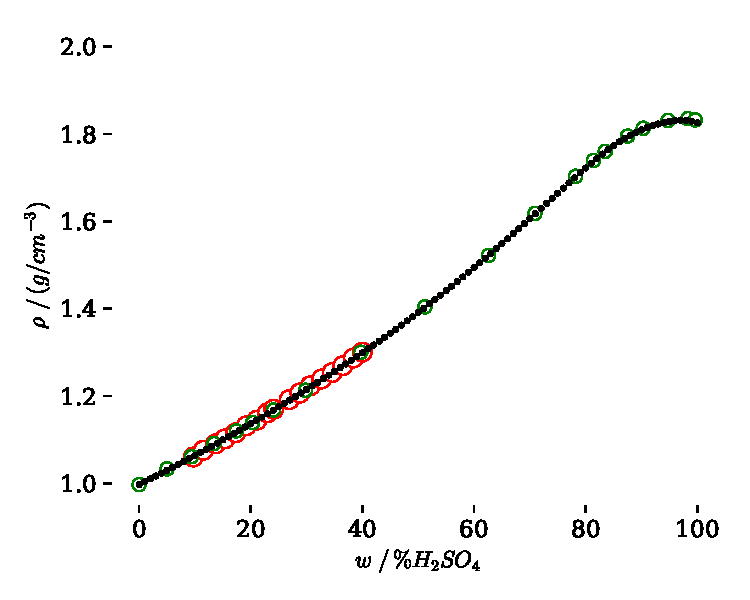
\includegraphics[scale=0.65]{images/plot_B1} 
  \label{fig:plotB1}
\end{figure}
\vspace{-10mm}

\begin{figure}
  \centering
  \caption[][10mm]{Plots of $\rho$ vs $w$ for data sets of Perry (small closed circles), Kaye (black open circles) and Oca (red circles) at \qty{20}{\degreeCelsius}\\ $\longleftarrow$} 
 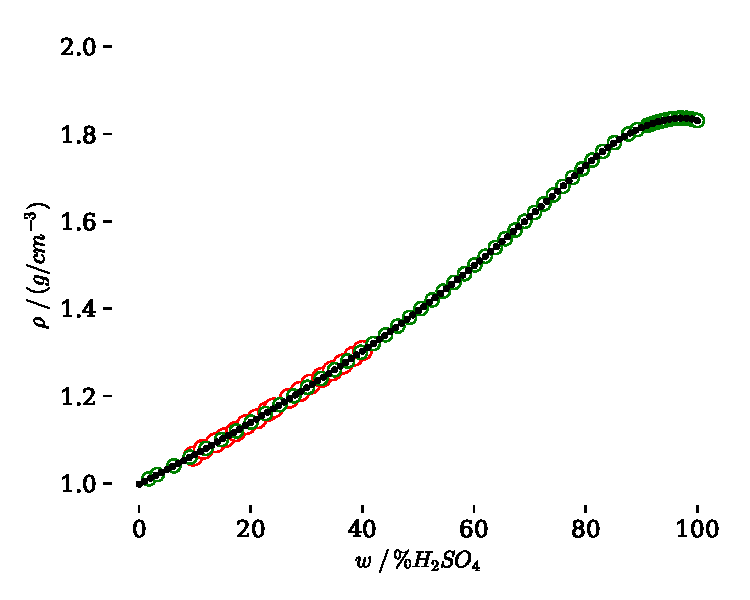
\includegraphics[scale=0.65]{images/plot_B2} 
  \label{fig:plotB2}
\end{figure}


\clearpage
\subsection{4\tss{th}-Degree Polynomial Fit}

A 4\tss{th}-degree polynomial model fits adequately, but we can do better. The data set was weighted at the ends to try to force a better fit\sidenote[][-10mm]{All of the details are presented in the code that generated the plot in Figure~\vref{fig:plotB5} and it is available in the \textit{Python} notebook. See reference \vref{ref:modelpython}. %For example, the concentration data used by Hyvärinen et al. was in mole percent, not percent mass. I had to convert it. You can see exactly what I did in the notebook and can decide for yourself if I performed the calculations correctly. %We chemists are very proud of the physical methods that we present in the \textit{methods} sections of our publications. However, it is rare that the details of the math are given equal detail. Providing \textit{Python} (or \textit{R}) notebooks is a way to document exactly what you did. Explanations are not needed when the code is available.
} in the high concentration region (see lower left plot). 

\marginnote[5mm]{\textsc{Hyvärinen Model}: The equation used in the polynomial fit is\ldots \\ \vspace{2mm}
$$\rho = a_4 \chi^4 + a_3 \chi^3 + a_2 \chi^2 + a_1 \chi + a_0$$\\  \vspace{1mm} 
\noindent $\chi$ is mole fraction of \ce{H2SO4} and it returns the density, $\rho$, in \unit{\kilo\gram\per\meter\cubed}\\ \vspace{0mm}
\begin{align*}
a_0 &=  \num{997.05} & a_1 &=  \num{3420} \\
a_2 &=  \num{-7230} & a_3 &=  \num{9090} \\
a_4 &=  \num{-4410}
\end{align*}
}

The model of Hyvärinen deviated badly. The authors had used their own measured density data. I extracted the data and observed that the model fits its own data very well, within its bounds. The lesson is that polynomial models should never be used for extrapolation. The Hyvärinen model matches its data between \num{0.5} and \qty{84.5}{\percent\ce{H2SO4}}.  It will go off the rails outside of that range, as it should.

The experimental data of Hyvärinen deviated from that of Perry (and the other data sets) above \qty{60}{\percent\ce{H2SO4}}. The model outperformed my own polynomial fit until that point, and then it followed the deviant data and diverged. 

\begin{figure}
  \centering
  \caption{Plots a 4\tss{th}-degree polynomial model. \vspace{1mm}
  
\noindent \textsc{Top}: The top plot presents the data set from Perry as small closed circles. The polynomial fit is traced by the red line. The parameterized model of Hyvärinen is traced in green and the experimental data used to make the that model is shown in larger open green circles.

 \vspace{1mm}
\noindent \textsc{Lower Left}: This plot is a closeup of the highest concentration region.

\vspace{1mm}
\noindent \textsc{Lower Right}: This is the differential plot. We can see that our model deviates significantly (small closed black circles). The Hyvärinen model is worse (small closed green circles). However, when the differentials are calculated between the Hyvärinen model and the data that was used to build it, we see good agreement (large green open circles). \\ $\longleftarrow$
}
 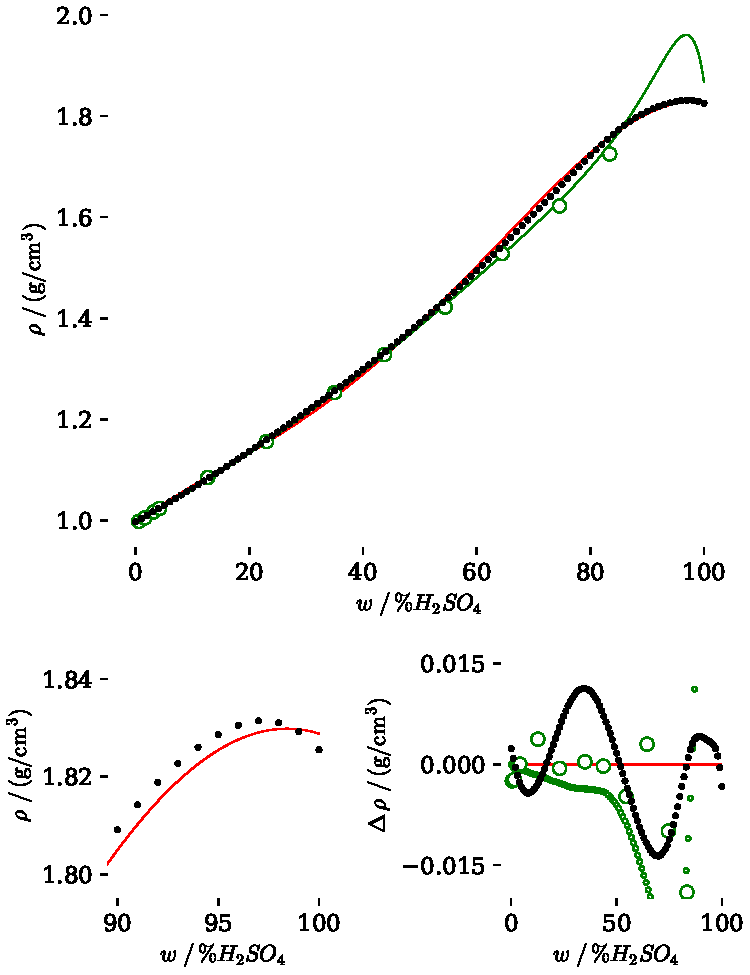
\includegraphics[scale=0.75]{images/plot_B5} 
  \label{fig:plotB5}
\end{figure}

\marginnote[-40mm]{\textsc{Polynomial Model}: The equation used in my own polynomial fit is\ldots \\ \vspace{2mm}
$$\rho = a_4 w^4 + a_3 w^3 + a_2 w^2 + a_1 w + a_0$$  

\noindent $w$ is \%\ce{H2SO4} and it returns the density, $\rho$, in \unit{\gram\per\centi\meter\cubed} \\ \vspace{0mm}
\begin{align*}
a_0 &=  \num{9.94729e-01} & a_1 &=  \num{8.29495e-03}\\
a_2 &=  \num{-1.30170e-04} & a_3 &=  \num{3.58003e-06} \\
a_4 &=  \num{-2.27374e-08}
\end{align*}
}
Next, we will try a six-parameter fit. Lets see how that improves the model. 



\clearpage
\subsection{6\tss{th} Degree Polynomial Fit}

A 6\tss{th}-degree polynomial model fits very well. the differentials are much smaller, but we will never eliminate the artifacts inherent in polynomial fits.\sidenote[][-10mm]{More parameters will make the deviations smaller and smaller. Try a 12-parameter fit using the \textit{Python} notebooks that I have provided.\tss{\ref{ref:modelpython}}} The data set was weighted at the ends.



\begin{figure}
  \centering
  \caption{Plots a 6\tss{th}-degree polynomial model. \vspace{1mm}
  
\noindent \textsc{Top}: The top plot presents the data set from Perry as small closed circles. The polynomial fit is traced by the red line (it fits the data so closely that it is hidden by the points. The parameterized model of Oca is traced in green. The experimental data used to make the model of Oca is shown in larger open green circles.

 \vspace{1mm}
\noindent \textsc{Lower Left}: This plot is a closeup of the highest concentration region.

\vspace{1mm}
\noindent \textsc{Lower Right}: This is the differential plot. We can see that our model is much closer to the data (small closed black circles). The differentials between the Oca model  and the Perry data set (small closed green circles) is also a great fit within the bounds of its data set. Again we see why we should never extrapolate with polynomial models. The differentials between the Oca model and the data that was used to build it show excellent agreement  (large green open circles). \\ $\longleftarrow$
}
 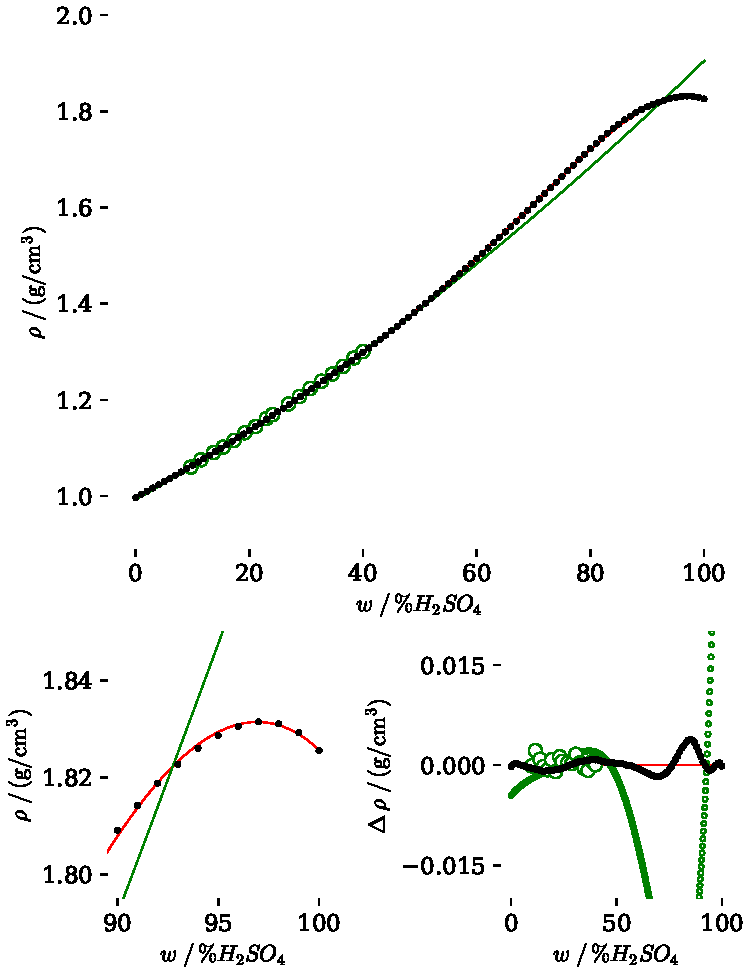
\includegraphics[scale=0.75]{images/plot_B5A} 
  \label{fig:plotB5A}
\end{figure}

\marginnote[-30mm]{\textsc{Oca Model}: The equation used in the poly\-nomial fit is\ldots 
\begin{multline*}
a_{0,0}\bar{w}^0T^0 + a_{0,1}\bar{w}^0T^1 + a_{0,2}\bar{w}^0T^2 \\+ a_{1,0}\bar{w}^1T^0 + a_{1,1}\bar{w}^1T^1 + a_{2,0}\bar{w}^2T^0
\end{multline*}
\vspace{0mm} 
\noindent $\bar{w}$ is mass fraction ($\nicefrac{w}{100}$) of \ce{H2SO4} and it returns the density, $\rho$, in \unit{\kilo\gram\per\meter\cubed}. $T = \qty{298.15}{\kelvin}$\\ \vspace{0mm}
\begin{align*}
a_{0,0} &=  \num{1122} & a_{0,1} &=  \num{-0.5076}\\
a_{0,2} &=  \num{2.484e-4} & a_{1,0} &=  \num{976.4} \\
a_{1,1} &=  \num{-1.015} & a_{2,0} &= \num{237.8} 
\end{align*}
}



\marginnote[-0mm]{\textsc{Polynomial Model}: The equation used in my own polynomial fit is\ldots \begin{multline*}
\rho = a_6 w^6 + a_5 w^5 + a_4 w^4 \\+ a_3 w^3 + a_2 w^2 + a_1 w + a_0
\end{multline*}
\noindent $w$ is \%\ce{H2SO4} and it returns the density, $\rho$, in \unit{\gram\per\centi\meter\cubed} \\ \vspace{0mm}
\begin{align*}
a_0 &=  \num{9.97298e-01} & a_1 &=  \num{6.34762e-03}\\
a_2 &=  \num{4.29036e-05} & a_3 &=  \num{-6.35832e-07} \\
a_4 &=  \num{3.16815e-09} & a_5 &= \num{1.74392e-10} \\
a_6 &= \num{-1.66035e-12}
\end{align*}
}


The Oca model is really a second degree polynomial w.r.t each of mass fraction ($\bar{w}$) and temperature ($T$). We chose a fixed temperature of \qty{25}{\degreeCelsius}. It is a three-parameter model and will not fit the entire range of the data from Perry. It performs adequately in the range of \num{0} to \qty{40}{\percent\ce{H2SO4}}, but fails quickly if you venture outside the range of data used to create it. 

The 6\tss{th}-degree polynomial model is a seven-parameter fit and does an excellent job of staying close to the training data.
      

%\subsection{Summary, So Far}

We have completed the second goal of this exercise: we can make polynomial models that relate concentration to density for sulphuric acid mixtures and have compared these models to literature models. I conclude that it is best to fit my own bespoke models rather than rely on literature polynomial models. As we have seen, there are more sophisticated models available in the literature that predict density across a wide range of temperatures and concentrations. I did not evaluate those --- I'm not going to transcribe 25 or 75 parameters. I'll role my own models using data sets that align with my needs.

\subsection{A Spline Fit}

After completing this exercise (see below) I learned a lot about fitting literature data tables. These tables were created using a parameterized model and are usually closely spaced in the series. the tables for $\rho$ are a good example of this. I can spend a lot of mental energy on these polynomial fits and their validation, or I can accept the data as it is and perform a simple interpolation. If the data is closely spaced along both the $x$ and $y$-axes then this will be the best option. Figure~\vref{fig:plot_B6} demonstrates a line created using a spline interpolation. More on this method will be presented later in this document. I have travelled back from the last page to add this information here.

\begin{figure}
  \centering
  \caption{Plots $H_0$ vs $m$ (\unit{\percent\ce{H2SO4}}) for the data of Gillespie and Johnson combined. Where duplicate values existed, the data from Gillespie was used. The spline interpolation is presented on the plot. This combined data set is precise and closely spaced so an interpolation is likely the best way to represent it.\\ $\longleftarrow$} 
  \hspace*{-10mm}
 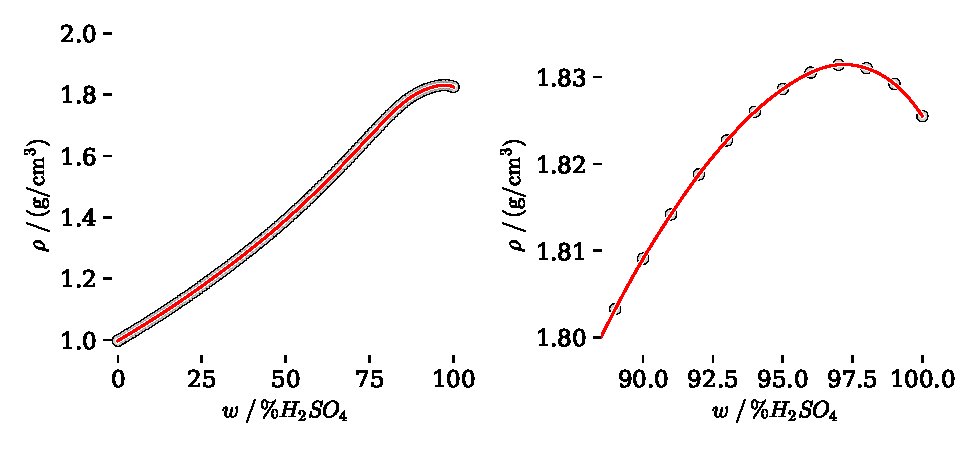
\includegraphics[scale=0.75]{images/plot_B6} 
  \label{fig:plot_B6}
\end{figure}


%%%%%%%%%%%%
%%%%%%%%%%%%
%%%%%%%%%%%%
%%%%%%%%%%%%

\section{3. A Model for $a_{H_2O}$ vs \%\ce{H2SO4}}

We will now move on to our third goal, constructing a model to predict $a_{H_2O}$ at any given concentration of a sulphuric acid-water mixture. I have data sets for this relationship from publications by Giauque\tss{\ref{ref:giauque}}, Rard\tss{\ref{ref:rard}} and Staples.\tss{\ref{ref:staples}} First let us plot these data sets together to see if they agree.

Each data set reports values of $a_{H_2O}$ (as fractional vapour pressure of water, $\nicefrac{p_x}{p_0}$) against concentration of \ce{H2SO4} (as molal values).  I will convert concentration from $m$ to $w$ and plot $a_{H_2O}$ vs. $w$ to compare the data sets as shown in Figure~\vref{fig:plotC1C}.


\begin{figure}
  \centering
  \caption{Plots $a_{H_2O}$ vs $w$ for the data sets of Giauque (small closed black circles), Rard (medium open green circles), and Staples (large open red circles). \vspace{1mm} \\ $\longleftarrow$
}
 \includegraphics[scale=0.75]{images/plot_C1c} 
  \label{fig:plotC1C}
\end{figure}

We can see that the Giauque data set (black) is sparse at lower concentrations and contains data from \qty{9}{\percent} to \qty{100}{\percent\ce{H2SO4}}. The Rard data set (green) tracks perfectly with Giauque and contains more data points with a span from \qty{1}{\percent} to \qty{72}{\percent\ce{H2SO4}}. I suspect it was derived from the same parameterized model or used the same data sets to generate the model. The Staples data had more data for low concentrations and spanned from \qty{0.1}{\percent} to \qty{73}{\percent\ce{H2SO4}}. It tracked almost perfectly with the both Giauque and Rard at concentrations below \qty{60}{\percent\ce{H2SO4}}, but diverged slightly at higher concentrations.

I will combine the data sets from Rard and Giauques.\sidenote[][-10mm]{I might remove duplicate points, or I might not. The \textit{Python} notebooks will have the recipe for my data sauce. Not only will others be able to examine my exact method, I will also be able to see what I have done. One month from now I will have no clue what was done to create the model. I could write very detailed notes, or I could unambiguously describe process in the \textit{Python} code. See reference \vref{ref:modelpython}.} This will give me a data set for $a_{H_2O}$ vs $w$ that will cover from \qty{1}{\percent} to \qty{100}{\percent\ce{H2SO4}}. The results of Yates et al.\tss{\ref{ref:ref1}} were in the range of \qty{10}{\percent} to \qty{99}{\percent\ce{H2SO4}}, so that is all that I need.

\subsection{Fitting the Model}

I combined the data of Rard\tss{\ref{ref:rard}} and Giauque\tss{\ref{ref:giauque}} by concatenating and sorting the data sets. I weighted the last ten points. See Figure~\vref{fig:plot_D1} for the results of this extreme polynomial fit.

\begin{figure}
  \centering
  \caption{Plots a 20\tss{th}-degree polynomial model for $a_{H_2O}$. \vspace{1mm}
  
\noindent \textsc{Top}: The top plot presents the data set from the combined data sets of Rard and Giauque for $a_{H_2O}$ vs $w$. The red line is calculated from the polynomial fit parameters. 

 \vspace{1mm}
\noindent \textsc{Lower Left}: This plot is a closeup of the highest concentration region.

\vspace{1mm}
\noindent \textsc{Lower Right}: This is the differential plot (\% difference). The model fits very well until we enter the region with very small values of $a_{H_2O}$. The average error between predicted and measured values was about \num{e-5}. This is great for most of the plot where $a_{H_2O}>\num{e-2}$, it is a large error when the values of $a_{H_2O}$ fall below \num{e-4} and become enormous for the final value where $a_{H_2O} \approx \num{e-9}$ \\ $\longleftarrow$
}
 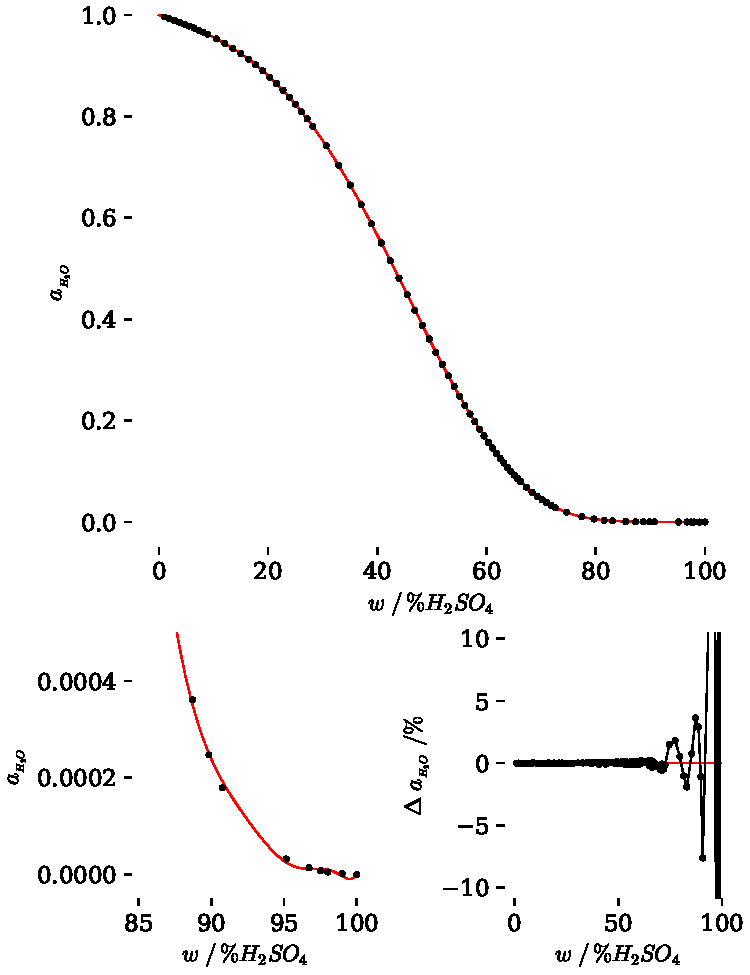
\includegraphics[scale=0.75]{images/plot_D1} 
  \label{fig:plot_D1}
\end{figure}

I was unable to obtain a model that provided an acceptable level of accuracy for predicting values of $a_{H_2O}$ in the high concentration region. As you can see, in desperation I used a 21-parameter fit. Still not good.

The range in the values is from 1 down to \num{e-9}. This is just too large of a change in magnitude. The fit is actually excellent with a median error of \num{8e-5}. But when data values are smaller than the error, we can have huge relative errors. The error in the final point is \qty{325}{\percent}

I tried lots of ways to improve the fit. Setting the weights to values of $\nicefrac{1}{a_{H_2O}}$ puts increasing weight toward the smaller values. this resulted in a fit that followed the data with \qty{2}{\percent} but the $Python$ numerical engine warned of errors. We needed such a high degree of a polynomial we were getting past the limits of double-floating point precision. 

\clearpage
\subsection{A Piecewise Model}

I tried splitting the data up into three sections and performing a piecewise fit. Each section still required high degrees of parameterization to get an adequate fit. Table~\ref{tab:piecewise} describes regions and models that were used.

\begin{table}[h!]
\caption{Pieces for the piecewise model. Small piece require fewer terms for an accurate fit. }
\centering


\label{tab:piecewise}
    \begin{tabular}{ccSS}
%        \toprule
        {$x$ Range \unit{\percent\ce{H2SO4}}} & {$y$ range}&{\# of Points} & {Degree}     \\
        \midrule
{$0 \le w < \qty{60}{\percent}$}& {1 to \num{e-1}}  & 62 & 12  \\ 
{$60 \le w < 85$}               &  {\num{e-1} to \num{e-3}} & 28 & 8   \\
{$ w \ge \qty{85}{\percent}$}   &  {\num{e-3} to \num{e-9}} & 11 & 6   
%        \bottomrule
    \end{tabular}
\end{table}

The piecewise polynomeial fit is displayed in Figure~\vref{fig:plot_D2}. It fits very well with most relative deviations between predicted and given data points being less that \qty{0.05}{\percent}. The largest relative error was at the final data point. The magnitude of that point was \num{e-9} and we hit it within a relative error of about \qty{1}{\percent}. 

\begin{figure}
  \centering
  \caption{Plots a piecewise polynomial model for $a_{H_2O}$. \vspace{1mm}
  
\noindent \textsc{Top}: The top plot presents the data set from the combined data sets of Rard and Giauque for $a_{H_2O}$ vs $w$. The thick transparent red line is calculated from the piecewise polynomial fit parameters. The piecewise polynomials that were used are also plotted. You can see why we never extrapolate with polynomials. Each was precise only within its assigned range: $0 \le x < 60$ (green), $60 \le x < 85$ (blue), and $x \ge 85$ (purple).

 \vspace{1mm}
\noindent \textsc{Lower Left}: This plot is a closeup of the highest concentration region. We observe an excellent fit using the 6\tss{th}-degree polynomial fit in the region where $x \ge 85$.

\vspace{1mm}
\noindent \textsc{Lower Right}: This is the differential plot (\% difference). The model fits very well until we enter the region with very small values of $a_{H_2O}$. The relative error only becomes visible toward the end of the plot. the average error for the final piece in the range $x \ge 85$ was \qty{0.1}{\percent}. The relative error for the final point was \qty{-1.1}{\percent}. \\ $\longleftarrow$
}
 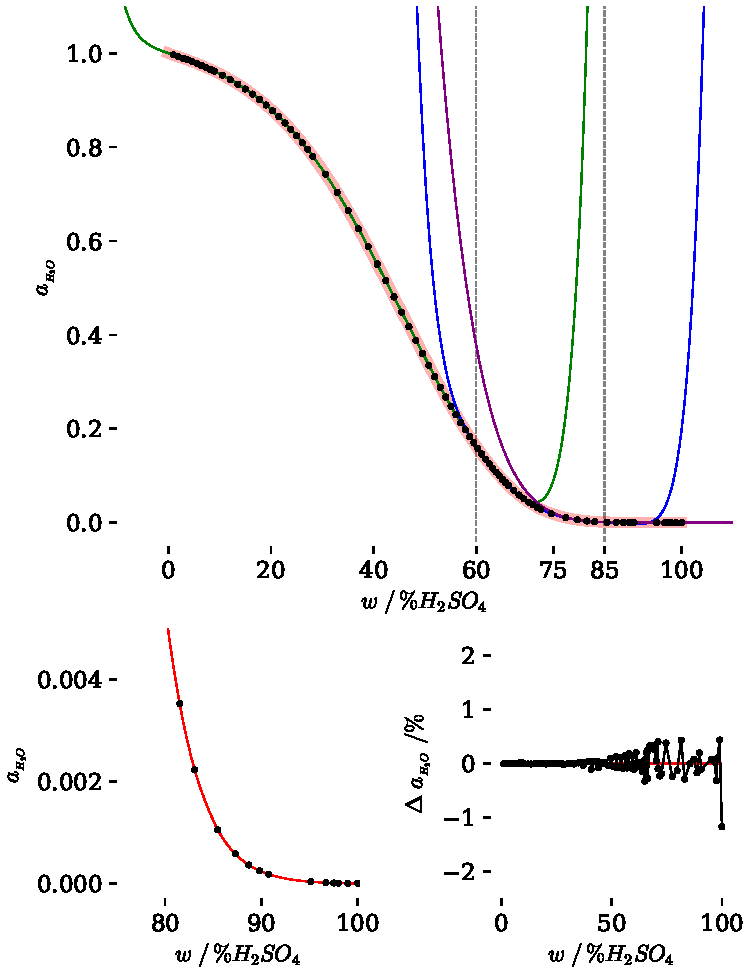
\includegraphics[scale=0.75]{images/plot_D2} 
  \label{fig:plot_D2}
\end{figure}

In a span of predicted values $10^0$ to \num{e-9}, we stayed very close to the given values. 

\subsection{Describing the Piecewise Function}

The model consists of three polynomials of degrees 12, 8 and 6 used in the regions of $w<\qty{60}{\percent}$, $\qty{60}{\percent} \le w < \qty{85}{\percent}$, and $w \ge \qty{85}{\percent}$.

\begin{equation} 
f(x) = \begin{cases}
    w<\qty{60}{\percent} & \displaystyle\sum_{n=0}^{12} a_n x^n \\
    \qty{60}{\percent} \le w < \qty{85}{\percent} & \displaystyle\sum_{n=0}^{8} b_n x^n \\
    w \ge \qty{85}{\percent} & \displaystyle\sum_{n=0}^{6} c_n x^n \\
    % ... and so on for more cases
\end{cases}
\end{equation}

The values for the coefficients are given in Table~\vref{tab:pieces}. Take note of the extreme degree of precision expressed. These high degree of the polynomials and the large range of magnitude in the values require every digit of precision that a 64-bit float can provide.

\begin{table}[h!]
\caption{Pieces for the piecewise model. Small piece require fewer terms for an accurate fit. \\ $\longleftarrow$ \\ \vspace{2mm} The high precision in these numbers is needed. Try rounding them off to eight digits and watch the fit wander far away from the given values.}
\centering


\label{tab:pieces}
\footnotesize
    \begin{tabular}{cl}
%        \toprule
        {Coefficient} & {Value} \\
        \midrule
{$a_0$}  & \num{9.999602819100265e-01}   \\
{$a_1$}  & \num{-3.75839371793719e-03}   \\
{$a_2$}  & \num{7.228976593850476e-05}   \\
{$a_3$}  & \num{-3.2632125447469756e-05}   \\
{$a_4$}  & \num{3.9261313528507605e-06}   \\
{$a_5$}  & \num{-3.2658573460234344e-07}  \\
{$a_6$}  & \num{1.7536108298451186e-08} \\
{$a_7$}  & \num{-6.266897770870015e-10}  \\
{$a_8$}  & \num{1.5036351730947478e-11}  \\
{$a_9$}  & \num{-2.3864159015620214e-13}  \\
{$a_{10}$} & \num{2.400749367443683e-15}  \\
{$a_{11}$} & \num{-1.3865886286472502e-17}  \\
{$a_{12}$} & \num{3.5028296585578643e-20}  \\
\midrule
{$b_0$} & \num{5.278125388514924e03}   \\ 
{$b_1$} & \num{-5.699778844885892e02}   \\ 
{$b_2$} & \num{2.683568358232527e01}   \\ 
{$b_3$} & \num{-7.193893888613687e-01}   \\ 
{$b_4$} & \num{1.200962559880584e-02}   \\ 
{$b_5$} & \num{-1.278611615731464e-04}   \\ 
{$b_6$} & \num{8.478783316886211e-07}   \\ 
{$b_7$} & \num{-3.2021412494451217e-09}   \\ 
{$b_8$} & \num{5.273726317476769e-12}   \\ 
\midrule 
{$c_0$} & \num{1.1164785064569885e02}   \\ 
{$c_1$} & \num{-6.8695694477137055e00}   \\ 
{$c_2$} & \num{1.762746136695284e-01}   \\ 
{$c_3$} & \num{-2.414407034715221e-03}  \\ 
{$c_4$} & \num{1.8616082649198916e-05} \\ 
{$c_5$} & \num{-7.660823213573518e-08} \\
{$c_6$} & \num{1.3144404858464668e-10} \\
%        \bottomrule
    \end{tabular}
\end{table}

Good luck typing all that in. I do not believe that I acheived my goal of a text-based, portable expression of the polynomial model. It is text, but it's not very easy to carry.
\clearpage

\subsection{Using $\log{a_{H_2O}}$ Values for the Model}

The huge range in values for $a_{H_2O}$ was too much for a simple polynomial fit, and is on the edge of possible for the piecewise model that I used above (there are better ways to do that. I am not an expert).

The values of $\log{a_{H_2O}}$ would have a dynamic range of less than one order of magnitude. Can I create a polynomial plot that predicts $\log{a_{H_2O}}$ vs \unit{{\percent\ce{H2SO4}}}?

\begin{figure}
  \centering
  \caption{Plots a polynomial model for $\log{a_{H_2O}}$. \vspace{1mm}
  
\noindent \textsc{Top}: The top plot presents the data set from the combined data sets of Rard and Giauque for $\log{a_{H_2O}}$ vs $w$. The red line is a 12\tss{th}-degree polynomial fit. It was not a satisfying result.

 \vspace{1mm}
\noindent \textsc{Lower Left}: This plot is a closeup of the highest concentration region. We observe a poor fit using the 12\tss{th}-degree polynomial fit in the region where $x \ge 85$. Remember that, on a log scale, a difference of ~1 is equivalent to an error of 10-fold (\qty{1000}{\percent}).

\vspace{1mm}
\noindent \textsc{Lower Right}: This is the differential plot. The model fits poorly across the whole range. A difference of 0.01 in $\log{a_{H_2O}}$ is the same as a \qty{25}{\percent} error in the predicted value for $a_{H_2O}$.  \\ $\longleftarrow$
}
 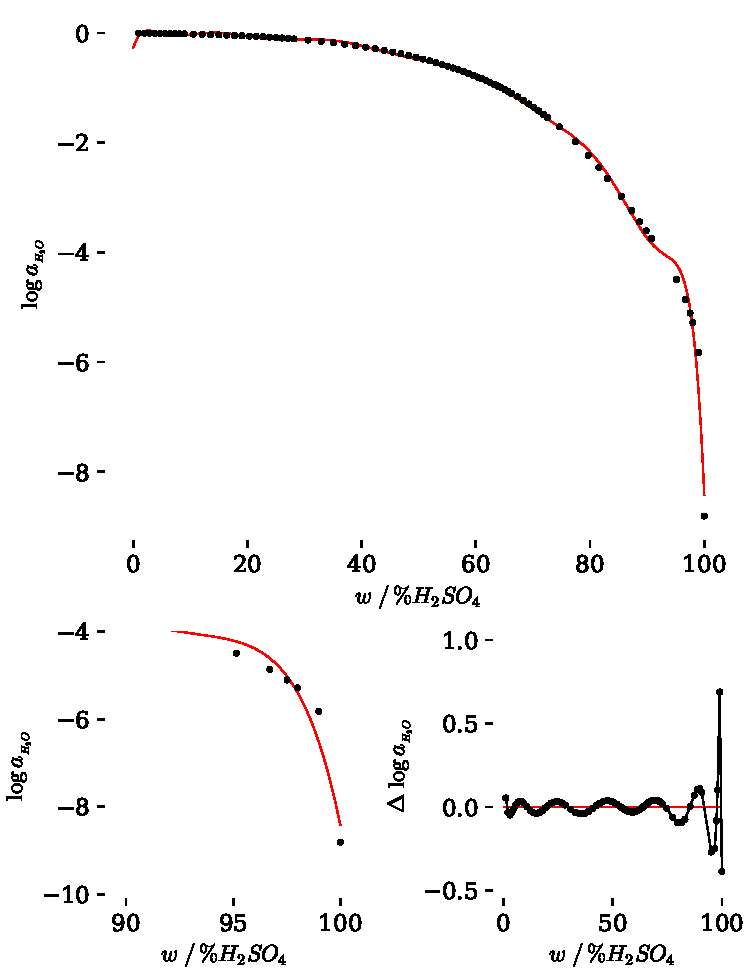
\includegraphics[scale=0.75]{images/plot_D3} 
  \label{fig:plot_D3}
\end{figure}

Clearly, my amateur efforts have failed. For whatever reason, the shape of the $\log{a_{H_2O}}$ vs \unit{\percent\ce{H2SO4}} curve defies a good polynomial fit. The large change between the last and second-last values again result in a poor fit. We do not have balanced data. The extremely steep slope at the end means that small imperfections in the model will yield large differences in the prediction. this high-concentration region was the most important in my analysis.

\clearpage

\subsection{Using Python Interpolation Functions}

I am using a polynomial fit to make a model for data that was likely derived from an undocumented polynomial model (at least, I haven't found the description yet). Perhaps I should just interpolate between the points.

\begin{figure}
  \centering
  \caption{Plots of \textit{Python} interpolation functions compared to the polynomial model for $\log{a_{H_2O}}$. \vspace{1mm}
  
\noindent \textsc{Top}: The top plot presents the data set from the combined data sets of Rard and Giauque for $a_{H_2O}$ vs $w$. The blue line is an interpolation function based on Bsplines. It is essentially a piecewise polynomial fit with many, many pieces.

 \vspace{1mm}
\noindent \textsc{Middle and Lower Left}: These plots are magnifications of the high concentration regions where the greatest difference in magnitude for values of $a_{H_2O}$ occur. Observe that a linear interpolation (green line, connect-the-dots) results in large relative errors when there is a significant span between points. My piecewise plot (red) and the interpolation function (blue) are nearly identical.

\vspace{1mm}
\noindent \textsc{Middle and Lower Right}: These are the corresponding relative differential plots. It is interesting to observe that the Bspline interpolation tracks very closely to the piecewise polynomial fit (3 pieces) that I had hacked together.  \\ $\longleftarrow$ \\ \vspace{5mm}

\noindent \textsc{Note}: The relative deviation between my own piecewise polynomial model and the spline interpolation is insignificant below \qty{60}{\percent\ce{H2SO4}}. At higher concentrations, as the value of $a_{H_2O}$ becomes very small, the relative deviations increase. The maximum deviations occur only at the highest concentrations of \ce{H2SO4} and are less than $\pm$\qty{5}{\percent}. The linear deviations for the linear interpolation are much greater, especially when there are larger spans between values and become unacceptable above \qty{90}{\percent\ce{H2SO4}}. 
}
 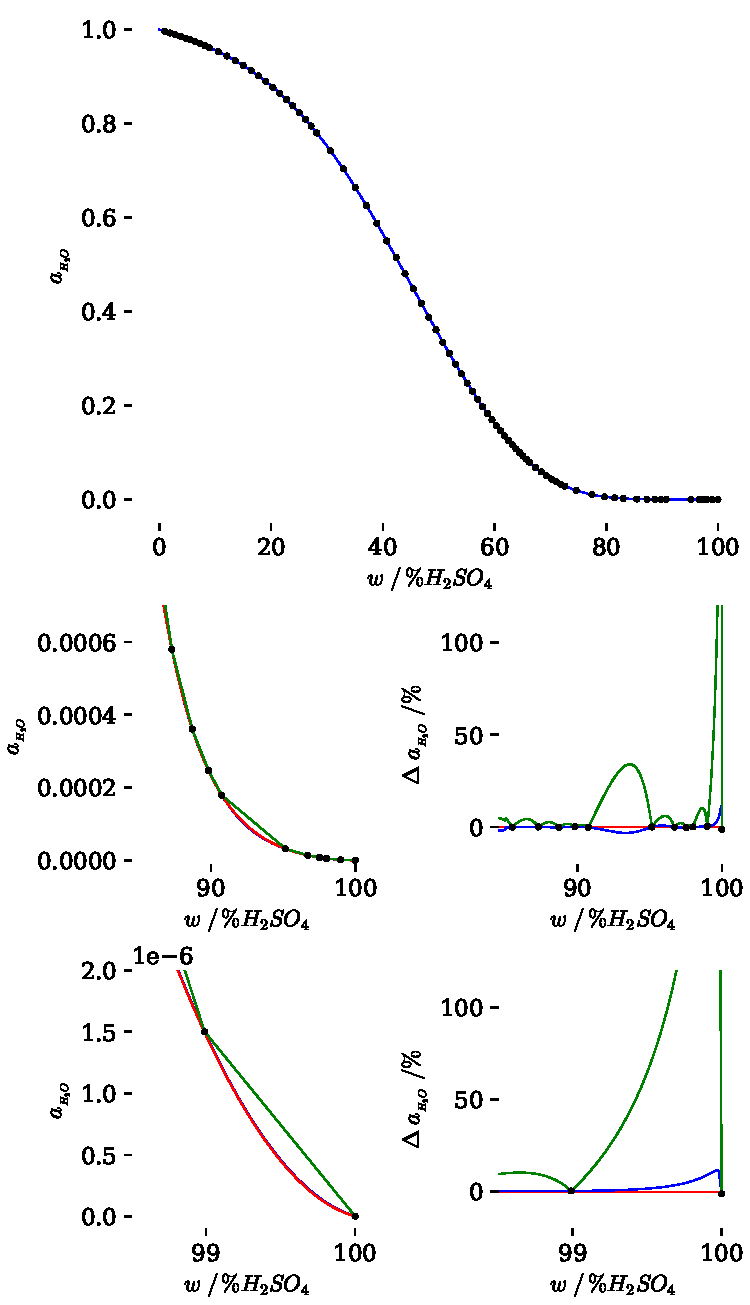
\includegraphics[scale=0.75]{images/plot_D4} 
  \label{fig:plot_D4}
\end{figure}

The model would simply be the data set and the python command to return values from the interpolation function. That actually seems simpler and more portable than the text-based description of my polynomial model in Table~\vref{tab:pieces}.

\clearpage

\section{4. A Model for $H_0$ vs \%\ce{H2SO4}}

Taking a lesson from all of the above wandering through various fits and interpolations I will now build a model to predict values of $H_0$ at any given value for $w$ (\unit{\percent\ce{H2SO4}}).

\begin{figure}
  \centering
  \caption{Plots $H_0$ vs $m$ (\unit{\percent\ce{H2SO4}}) for various data sets available in the literature. Data is from: Gillespie, 1971,\tss{\ref{ref:gillespie}} blue; Johnson, 1969,\tss{\ref{ref:johnson}} black; Jorgenson, 1963,\tss{\ref{ref:jorgenson}} red; Tickle, 1970,\tss{\ref{ref:tickle}} orange; Paul \& Long, 1953,\tss{\ref{ref:paul}} green\\ $\longleftarrow$} 
  \hspace*{-10mm}
 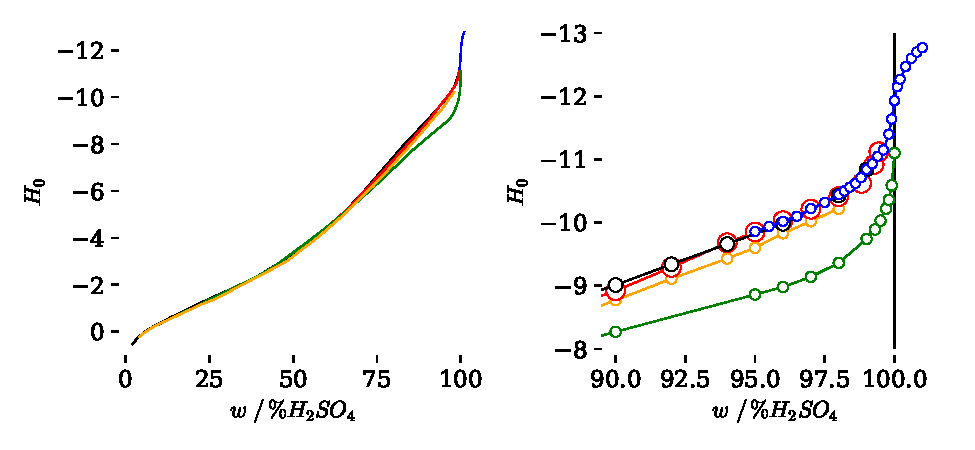
\includegraphics[scale=0.75]{images/plot_F1} 
  \label{fig:plot_F1}
\end{figure}
\vspace{-10mm}
\subsection{Assembling the Data}

The data reported by Gillespie et al.,\sidenote[][-30mm]{``Hammett acidity function for some super acid systems.'' R.J. Gillespie, T.E. Peel, and E.A. Robinson, \textit{J. Am. Chem. Soc.}, \textbf{1971}, \textit{93}, 5083-5087. \url{https://doi.org/10.1021/ja00749a021}\vspace{2mm}\label{ref:gillespie}} Johnson et al.,\sidenote[][-10mm]{``Temperature variation of the $H_0$ acidity function in aqueous sulfuric acid solution.'' C.D. Johnson, A.R. Katritzky, S.A. Shapiro \textit{J. Am. Chem. Soc.}, \textbf{1969}, \textit{91}, 6654-6662. \url{https://doi.org/10.1021/ja01052a021}\vspace{2mm}\label{ref:johnson}} and Jorgenson et al.,\sidenote[][0mm]{``A Critical Re-evaluation of the Hammett Acidity Function at Moderate and High Acid Concentrations of Sulfuric Acid. New $H_0$ Values Based Solely on a Set of Primary Aniline Indicators.''M.J. Jorgenson, D.R. Hartter, \textit{J. Am. Chem. Soc.}, \textbf{1963}, \textit{85}, 878-883. \url{https://doi.org/10.1021/ja00890a009}\vspace{2mm}\label{ref:jorgenson}} agreed closely. The values reported by Tickle et al.,\sidenote{P. Tickle, A.G. Briggs, J.M. Wilson, \textit{J. Chem. Soc. B}, \textbf{1970}, 65-70. \url{https://doi.org/10.1039/J29700000065}\vspace{2mm}\label{ref:tickle}} tracked closely with the above but were significantly different at higher concentrations. The values of Paul \& Long\sidenote[][0mm]{``$H_0$ And Related Indicator Acidity Functions.'' M.A. Paul, F.A. Long, \textit{Chem. Rev.}, \textbf{1957}, \textit{57}, 1-45. \url{https://doi.org/10.1021/cr50013a001}\vspace{2mm}\label{ref:paul}} diverged greatly above \qty{70}{\percent\ce{H2SO4}}.

All five data sets described above are clearly outputs of parameterized models fit to experimental data. I am sure the original data could be found in the literature, but I am not going to spend the time. The data sets of Johnson and of Jorgenson are nearly identical across their entire mutual range of 60 to \qty{99}{\percent\ce{H2SO4}}. Johnson covers a broad range from 2 to \qty{99}{\percent\ce{H2SO4}}. The data reported by Gillespie is at extreme concentrations of 95 to \qty{101}{\percent\ce{H2SO4}}\sidenote[][0mm]
{Your little-league coach was right. you can give more than \qty{100}{\percent}. At least that is true for sulphuric acid. Pure \ce{H2SO4} is, in fact, only \qty{98}{\percent\ce{H2SO4}}. This is due to the equilibrium dissociation of \ce{H2SO4} to give \ce{H2O} and \ce{SO3} (observe that \qty{100}{\percent} has a non-zero value for $a_{H_2O}$). What is called ``\qty{100}{\percent\ce{H2SO4}} is pure \ce{H2SO4} to which excess \ce{SO3} has been added. This is the famous ``fuming sulphuric acid.''} I will use these data sets to build my own model for $H_0$ vs $m$ from \num{2} to \qty{101}{\percent\ce{H2SO4}}.

One approach is to combine the three data sets to train a polynomial model. I can use all the data and obtain the best fit. Or I could use a spline interpolation using selected data points that create a smooth set of precise points assembles in the order of increasing \unit{\percent\ce{H2SO4}}. 
\clearpage
\subsection{A Polynomial Model}

Again, I created a 12\tss{th}-degree polynomial model and fit it to the data. Figure~\vref{fig:plot_G2}. It diverged at the highest values of $m$. The differential plot shows how the fit followed between the Johnson and the Jorgenson data sets, and then began diverging as it moved into the Gillespie data at very high values of $w$. There are probably better ways to do this such as splitting it into pieces like before but I feel that interpolation will be the best option here.

\begin{figure}
  \centering
  \caption{Plots of the polynomial model for $H_0$ vs \unit{\percent\ce{H2SO4}} . \vspace{1mm}
  
\noindent \textsc{Top}: The top plot presents the data set from the combined data sets of Johnson, Jorgenson and Gillespie. The red line is a 12\tss{th}-degree polynomial fit. It was satisfactory at all but the most extreme concentrations.

 \vspace{1mm}
\noindent \textsc{Lower Left}: This plot is a closeup of the highest concentration region. We observe a divergence the region where $w >\qty{95}{\percent\ce{H2SO4}}$. Remember that, on a log scale, a difference of ~0.3 is equivalent to an error of two-fold (\qty{100}{\percent}).

\vspace{1mm}
\noindent \textsc{Lower Right}: This is the differential plot. The model fits adequately across the whole range with errors become excessive only above \qty{100}{\percent\ce{H2SO4}}.  \\ $\longleftarrow$
}
 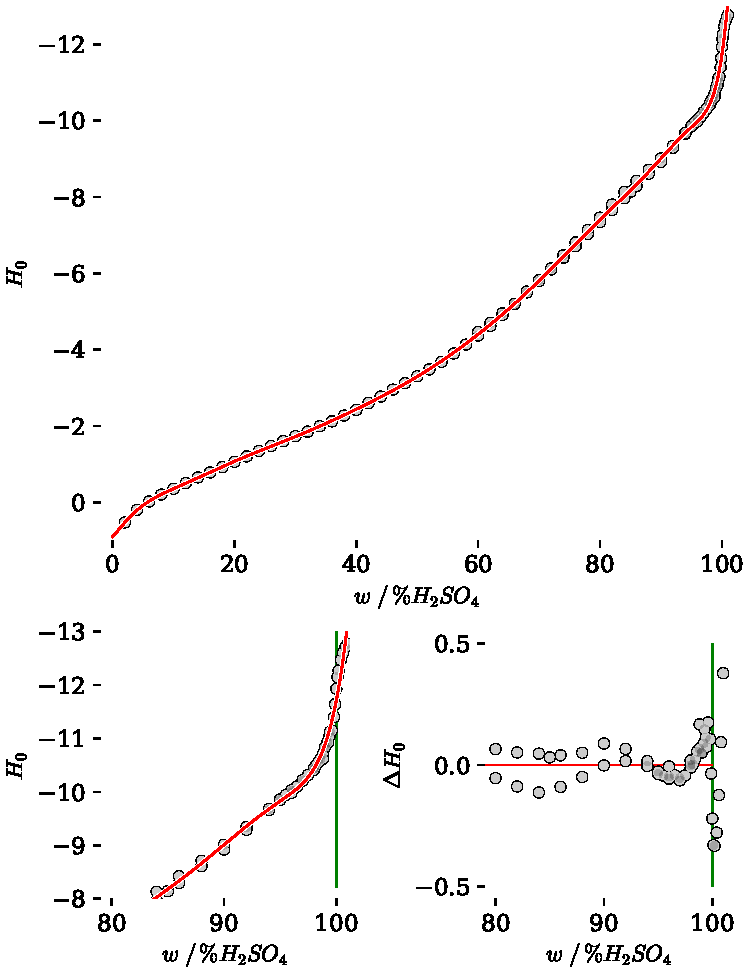
\includegraphics[scale=0.75]{images/plot_G2} 
  \label{fig:plot_G2}
\end{figure}

\subsection {An interpolated Model}

To use an interpolator it is required to have a set of single values on an increasing x-axis series. I could average the values where there are duplicates at a given value of $m$. I decided to use the Johnson and Gillespie data sets to cover the range from \num{2} to \qty{101}{\percent\ce{H2SO4}}. The data is precise and closely spaced and so the interpolation is a good representation of the data. Figure~\vref{fig:plot_G3} shows the result.

\begin{figure}
  \centering
  \caption{Plots $H_0$ vs $m$ (\unit{\percent\ce{H2SO4}}) for the data of Gillespie and Johnson combined. Where duplicate values existed, the data from Gillespie was used. The spline interpolation is presented on the plots. The right-hand plot is a detail region. This combined data set is precise and closely spaced, so an interpolation is likely the best way to represent it.\\ $\longleftarrow$} 
  \hspace*{-10mm}
 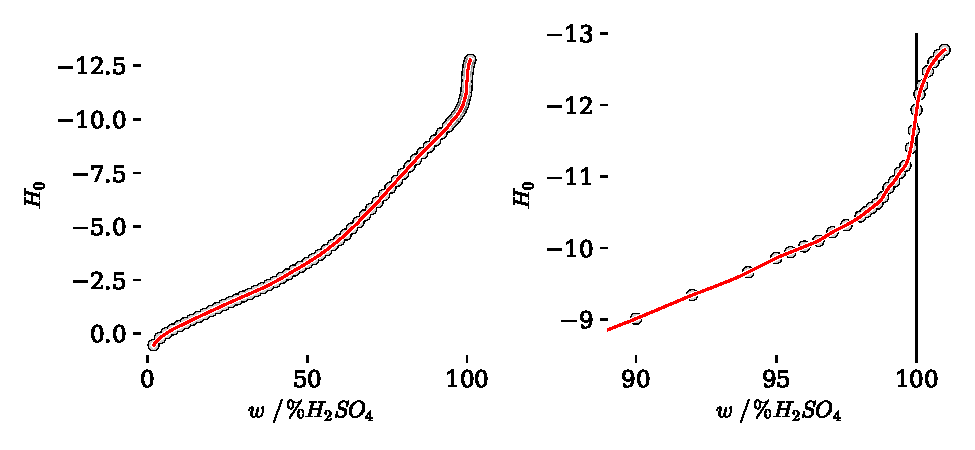
\includegraphics[scale=0.75]{images/plot_G3} 
  \label{fig:plot_G3}
\end{figure}

\section{Where Are We Now?}

What a long strange journey it has been. I began this exercise seeking a better way to interpolate the literature data sets for $\rho$, $a_{\ce{H2O}}$ \& $H_0$ of sulfuric acid mixtures. I was unhappy with the results of interpolation that I was using previously and wanted to try polynomial models for this interpolation. In the end I am all the way back to recommending a simple interpolation of the points in the data table as the solution for most cases. In the case of $a_{\ce{H2O}}$ values, where there is an enormous difference in magnitude between the final data points at high concentrations, the polynomial fit might be best. However, it was an complicated piecewise model requiring extreme precision in the parameters. The simple interpolation was good enough.

The reason that my interpolation for $a_{\ce{H2O}}$ was taking an excursion into negative values and causing errors in my calculations was because I had previously been using a smoothing interpolation function (useful for experimental data that contains random error). This did a little too much smoothing. I used a more traditional Bspline interpolator function, \texttt{SciPy.interpolate.\-make-interp-spline}, and it produced a better result. When someone says they interpolated their data, the exact method matters. You can see exactly what I have done by examining my \textit{Python} code for yourself.\sidenote[][-10mm]{Using \textit{Python} notebooks will enable you to ``show your work'' for any problem that you are solving. No need for long winded documents like this one.  See reference \vref{ref:modelpython}}

\section{5. Comparing Our $a_{\ce{H2O}}$ Against Cox}

The analysis that I have been using for the results of Yates and McClelland\tss{\ref{ref:ref1}} are based on a method called the ``excess acidity method.'' To use this method, we will need good values for $H_0$ and $a_{\ce{H2O}}$. Robin Cox, a longtime collaborator of Yates, published a review of the excess acidity method\tss{\ref{ref:cox}} in the year 2000 and, in that paper, produced tables of excess acidity values (related to $H_0$ values) and $a_{\ce{H2O}}$ values. I want to compare my values with those in the table by Cox.
\subsection{Converting Units}
The tables of $a_{\ce{H2O}}$ from Giauque\tss{\ref{ref:giauque}} and others are presented as fractional vapour pressures ($p_x / p+0$), but the values reported by Cox are in units of apparent molar concentration. I will need to obtain an activity coefficients from the value of  $a_{\ce{H2O}}$ and the formal mole fraction of \ce{H2O} and then multiply that against the formal molar concentration of \ce{H2O}. Will I get the same values?

I extracted activity coefficients for water in \ce{H2SO4} ($\gamma_w$) by using the formal mole fraction of water in the mixture ($x_w$) and the apparent mole fraction (fractional vapour pressure, $\nicefrac{p_x}{p_0}$ or $a_{H_2O}$. 

$$ \gamma_w = \frac{a_{H_2O}}{x_w} $$

I then calculated the formal molar concentration of water in the mixture using the interpolated density tables to convert $w$ (\unit{\percent\ce{H2SO4}}) to $M$ (\unit{\mol\per\litre}). The product of the activity coefficient and molar concentration will give the activity of water in units of molarity.

$$a_{H_2O}^M = \gamma_w [\ce{H2O}]$$

I converted the data set that I had assembled from Giauque\tss{\ref{ref:giauque}} and Rard\tss{\ref{ref:rard}} (see a plot of that data set in Figure~\vref{fig:plot_D4}) so that the values of $a_{H_2O}$ were in units of molarity. I designated this set of activity values as $a_{H_2O}^M$. 
\subsection{Comparing Cox and Giauque}
A plot of $a_{H_2O}^M$ vs $w$ for both the values that I had just converted and the values reported by Cox\tss{\ref{ref:cox}} is presented in Figure~\vref{fig:plot_H1}.

\begin{figure}
  \centering
  \caption{Plots of $a_{H_2O}^M$ (\unit{\mole\per\litre}) vs $m$ (\unit{\percent\ce{H2SO4}}) for the data of Giauque and Rard combined (black) along with the data set presented by Cox (red, Table 3 in the paper; blue, Table 4). The green line is the calculated formal concentration of \ce{H2O} in the mixture.\\ $\longleftarrow$} 
%  \hspace*{-10mm}
 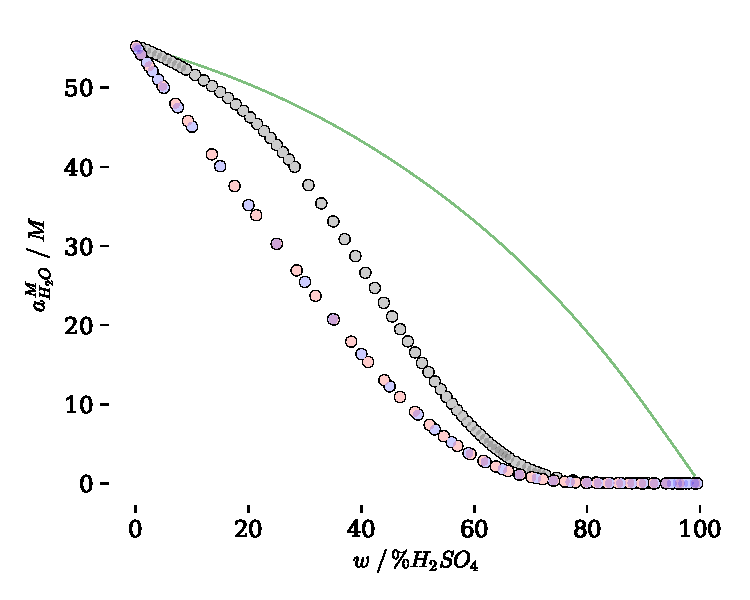
\includegraphics[scale=0.75]{images/plot_H1} 
  \label{fig:plot_H1}
\end{figure}

We can clearly see that the values for $a_{H_2O}^M$ that were used by Cox are different than the ones derived from Giauque and Rard. The values above \qty{70}{\percent\ce{H2SO4}} are not able to be separated from each other. Plotting using a log scale will be more useful. The plot of $\log{a_{H_2O}^M}$ vs $w$ is presented in Figure~\ref{fig:plot_H2}. I observe that the difference is less than an order of magnitude throughout most of the range, with the deviation being about 0.3 to 0.4 log units (the values for $a_{H_2O}^M$ used by Cox are about one half of those from Giauque and Rard). This is not really a big difference in the world of physical organic chemistry, but I still need to explain it.

\begin{figure}
  \centering
  \caption{Plots of $\log{a_{H_2O}^M}$ (\unit{\mole\per\litre}) vs $m$ (\unit{\percent\ce{H2SO4}}) for the data of Giauque and Rard combined (black) along with the data set presented by Cox (red, Table 3 in the paper; blue, Table 4). The green line is the calculated formal concentration of \ce{H2O} in the mixture. The black line is data calculated from osmotic activities reported by Zeleznick.\\ $\longleftarrow$} 
%  \hspace*{-10mm}
 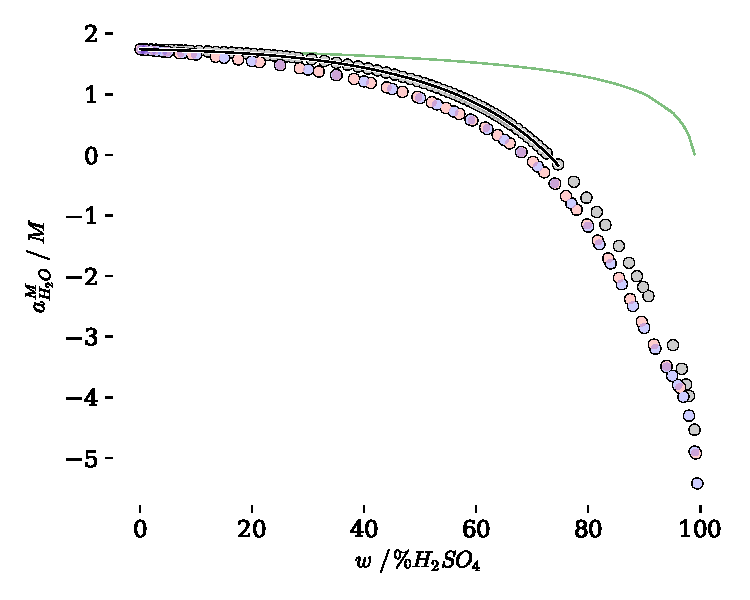
\includegraphics[scale=0.75]{images/plot_H3} 
  \label{fig:plot_H2}
\end{figure}

\subsection{Investigating the Data Sources}
The review by Cox\tss{\ref{ref:cox}} was written in the year 2000. The data that we will be considering that was presented by Yates and McClellan\tss{\ref{ref:ref1}} is from 1967 and the values they used for $a_{H_2O}$ were from Giauque\tss{\ref{ref:giauque}} in 1960. Cox had access to more recent data for values of $a_{H_2O}$. He used a data set presented by Frank Zeleznik\sidenote[][0mm]{``Thermodynamic Properties of the Aqueous Sulfuric Acid System to 350 K.'' F.J. Zeleznik, \textit{J. Phys. Chem. Ref. Data} \textbf{1991} \textit{20}, 1157–1200. \url{https://doi.org/10.1063/1.555899}. Obtained via inter-library loan. You can also access the paper via \url{https://www.nist.gov/system/files/documents/srd/jpcrd426.pdf}. I eventually found a better copys at \url{https://srd.nist.gov/jpcrdreprint/1.555899.pdf}. Both of those are US government sources, so I presume that they are freely available.\label{ref:zeleznick}\vspace{2mm}} in 1991. The data presented in Table~8 of that paper reported the osmotic coefficient vs molal concentration for sulphuric acid/water mixtures up to \qty{30}{\mole\per\kilo\gram} (\qty{75}{\percent\ce{H2SO4}}). Osmotic coefficients are a common way to determine values for $a_{H_2O}$ and I converted these values to units of activity as partial pressure using the standard equation\sidenote[][0mm]{``Thermodynamic Properties of Aqueous Sulfuric Acid.'' H. Sippola, P. Taskinen, 
\textit{J. Chem. Eng. Data}, \textbf{2014}, \text{59},  2389-2407. \url{https://doi.org/10.1021/je4011147}\label{ref:sippola}\vspace{2mm}} displayed below as eq.~\ref{eq:osmosis}.  

\begin{equation}\phi = -\left(\frac{1000}{M_W \nu m}\right)\ln{a_{H_2O}}\label{eq:osmosis}\end{equation}


Where the osmotic coefficient, $\phi$ is defined in terms of $a_{H_2O}$ ($\nicefrac{p_x}{p_0}$). $M_W$ is the molar mass of water, \qty{18.015}{\gram\per\mole}; $\nu$ is the number of ions that sulfuric acid can produce on complete dissociation ($\nu = 3$ in this case); and $m$ is the concentration of \ce{H2SO4} in molal units.

I plotted values of $a_{H_2O}^M$ calculated from the osmotic coefficient data of Zeleznick. It is presented as the black line in Figure~\vref{fig:plot_H2} and I observed that it tracked perfectly with the data of Giauque and Rard and not with the values reported by Cox. 

\subsection{Digging Deeper}
So where did Cox get his data for $a_{H_2O}^M$? The Zeleznick paper reports the osmotic coefficients only to \qty{75}{\percent\ce{H2SO4}} and the data table of Cox goes to \qty{99}{\percent}. Cox did not report $a_{H_2O}^M$ calculated from the osmotic coefficient data data table, but used the parameterized curve fit model described in the paper. There is no model for osmotic coefficients in the paper so I had to read it carefully and not just look at the pictures and the data tables.

The model that is proposed by Zeleznick is completely inscrutable to me. The photocopy of the paper that I obtained vie interlibrary loan had about half and inch cut of along the text on the sides of each page. Some terms in the equations are this missing. Even if I wanted to get into the weeds with this model, it has 50 parameters and uses a complex algorithm with three summation loops. If someone can get me a good copy of page~1185 and help me parse through equations 11, 12 and 13 of the Zeleznick paper\tss{\ref{ref:zeleznick}}, please contact me.\sidenote[][0mm]{I eventually found a better copy of the paper and could follow the equation now, but I think I still need help.\vspace{2mm}} I tried following the trail of references to the papers where Zeleznick first presented these equations\sidenote[][0mm]{``A class of nonideal solutions. 1: Definition and properties.'' F.J. Zeleznick, \textit{NASA TP-1929}, \textbf{1983}. \url{https://ntrs.nasa.gov/citations/19830014918}\vspace{2mm}}\tss{,}\sidenote[][0mm]{``A class of nonideal solutions. 2: Application to experimental data'' F.J. Zeleznick, L.F. Donovan, \textit{NASA TP-1930}, \textbf{1983}. \url{https://ntrs.nasa.gov/citations/19830014917}\vspace{2mm}}
 but these were intense works of mathematics and completely defeated me.
 
\subsection{Using the Pictures} 

Zeleznick used his model to calculate the relative chemical potential for water in sulphuric acid, $\mu_1 - \mu_1^*$ where $\mu_1$ is the chemical potential for a water-sulphuric acid mixture and $\mu_1^*$ is the chemical potential for the standard state of water. From this value, the osmotic coefficient, $\phi$, was calculated according to Eq.~\vref{eq:zel11} and then the value of $a_{H_2O}$ can be calculated using Eq.~\vref{eq:osmosis}.

\begin{equation}
\frac{\mu_1 - \mu_1^*}{RT} = 3\frac{x_1}{x_2}\phi
\label{eq:zel11}\end{equation}

Zeleznick presents values of osmotic coefficients, $\phi$, that were calculated using his model in Table~8 of his paper. But Cox must have used his model and calculated values of $\mu_1 - \mu_1^*$ and then converted these to values of $a_{H_2O}^M$. I have tries using the equations for a few data points and do not get anything near what is reported by Zeleznick. I'm doing it wrong and don't know how to do it right. I see in Figure~25 of the paper that Zeleznick presents a graph of $-\nicefrac{\mu_1 - \mu_1^*}{RT}$ values for sulphuric acid and water. I have reproduced this graph in Figure~\vref{fig:scanned}. Zeleznick presents data calculated to \qty{99.5}{\percent}. The data in his Table~8 gives me data only to a mole fraction of 0.35 (\qty{75}{\percent}).

\begin{figure}
  \centering
  \caption{Plots of $-\nicefrac{\mu_1 - \mu_1^*}{RT}$ vs mole fraction \ce{H2SO4} for values calculated from the models of Zeleznick and Giauque. I have added indications for values of concentration in units of $w$, \unit{\percent\ce{H2SO4}}, for comparison sake. I observe that the values are nearly identical to those of Giauque until we exceed a mole fraction of 0.5 (\qty{85}{\percent\ce{H2SO4}}).\\ $\longleftarrow$}
%  \hspace*{-10mm}
 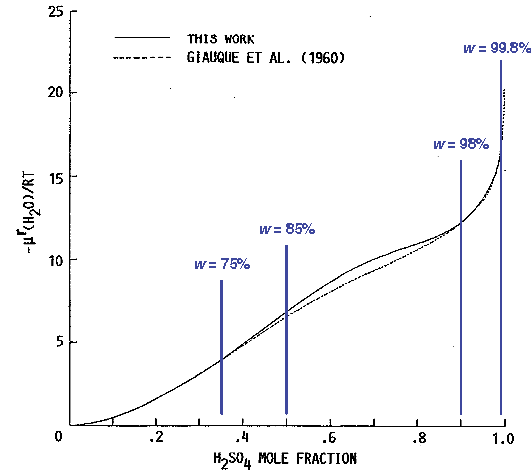
\includegraphics[scale=1]{images/ZeleznickFig25B.pdf} 
  \label{fig:scanned}
\end{figure}

I will use a plot digitizer\sidenote[][0mm]{I used WebPlotDigitizer by Ankit Rohatgi. \url{https://automeris.io/v4/}\vspace{2mm}} to extract a set of points from the line drawn by Zeleznick for his own calculated results. I can compare my extracted results to those derived from his table of osmotic coefficients. The data extracted is values for $-\nicefrac{\mu_1 - \mu_1^*}{RT}$. Using Eq.~\ref{eq:zel11} as reported by Zeleznick did not give correct values for $\phi$. My physical chemistry is weak, but I do know that there is no need to convert chemical potential to osmotic coefficients and then to activity. Activity can be calculated directly from the chemical potential.\sidenote[][0mm]{Recall that chemical potential of a reactant is actually a measure of the activity of a component as expressed by the activity coefficient and concentration, $a_x = \gamma_x\cdot c_x$\vspace{2mm}} I will use the formula for calculating activity from the difference between the chemical potential in the standard state and that observed in the given system.\sidenote[][0mm]{`activity'' in \textit{IUPAC Compendium of Chemical Terminology}, 5\tss{th} ed. International Union of Pure and Applied Chemistry, \textbf{2025}. Online version 5.0.0, 2025. \url{https://doi.org/10.1351/goldbook.A00115}\vspace{2mm}} as shown in Eq.~\vref{eq:iupac}.

\begin{equation}
a_x = e^{\frac{\mu_x - \mu_x^*}{RT}} 
\label{eq:iupac}\end{equation}

I now have a set of data for chemical potentials of water as calculated from the models of Giauque and of Zeleznick according to Figure~25B in Zeleznick's paper.\tss{\ref{ref:zeleznick}} I converted the these chemical potential values to activity and then to molar activity for water and plotted the data in Figure~\vref{fig:scannedplot}. As you can see, the data tracked very well with the points that I had derived from Giauque's data tables previously. The potentials calculated from Zeleznick's model and presented in Figure~25B of the paper agreed almost perfectly with the Giauque data except in the region above \qty{85}{\percent\ce{H2SO4}}. 

\begin{figure}
  \centering
  \caption{Plots of $\log{a_{H_2O}^M}$ (\unit{\mole\per\litre}) vs $m$ (\unit{\percent\ce{H2SO4}}) derived from Figure~25B in Zeleznick.\tss{\ref{ref:zeleznick}}. \\ $\longleftarrow$ \\ \vspace{1mm}
  
\noindent Red solid line: the digitized data from Giaugue's model as presented in Zeleznick's figure.\\ \vspace{1mm}

\noindent Blue solid line: the digitized data from Zeleznick's model.\\ \vspace{1mm}
  
\noindent Green dashed line: The green line is the calculated formal concentration of \ce{H2O} in the mixture.\\ \vspace{1mm}
  
\noindent Black dashed line: The data of Giauque and Rard combined together (this line is mostly obscured by the red line). \\ \vspace{1mm}
  
\noindent Blue dashed line: the data set presented by Cox in Table 3 of his paper\tss{\ref{ref:cox}}.} 
%  \hspace*{-10mm}
 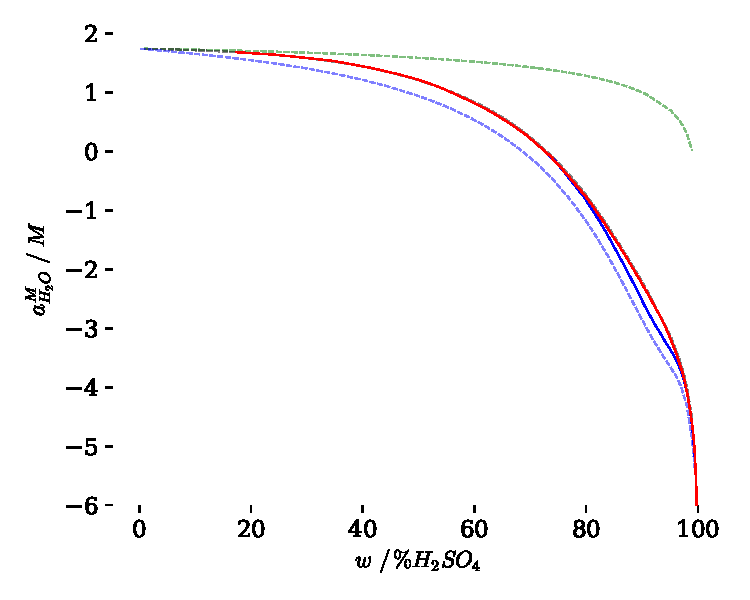
\includegraphics[scale=0.75]{images/plot_H4} 
  \label{fig:scannedplot}
\end{figure}

Zeleznick's discussion about the difference between his model and the model of Giauque expresses some frustration with a lack of information about the exact methodology and math in that model. Zeleznick proposes some possible reasons for the difference but cannot be sure as the math was not documented in detail. If only \textit{Python} notebooks had been available in 1960, alas.

I still cannot explain the difference between my calculated molar activity values for water and those of Cox. It is clear that he used the model of Zeleznick (observe how the Cox data set is nearly parallel with the Zeleznick model in the region above \qty{85}{\percent}) but there is a significant difference across the whole data set. I cannot explain this difference. I have no information about the math that was used by Cox but I suspect that the difference lies there. Cox states that he calculated the molar concentration of water using a standard equation found in Robinson and Stokes.\sidenote[][0mm]{``Electrolyte Solutions -- The Measurement and Interpretation of Conductance, Chemical Potential and Diffusion in Solutions of Simple Electrolytes. 2\tss{nd} ed.'' R. A. Robinson and R. H. Stokes,  \textbf{1970}, \textit{Dover Publications, Mineola, NY}, reprint edition, 2002. Page 31.\vspace{2mm}} This equation is the same one that I used. You can check my math, but we cannot check the math in the paper of Cox.\sidenote[][-0mm]{The \textit{Python} notebook for all following calculations and plots involving the data of Cox can accessed via Google Colab at \url{https://colab.research.google.com/github/blinkletter/4410PythonNotebooks/blob/main/Class_30_Yates_New/cox.ipynb}.\vspace{2mm}\label{ref:coxmodelpython} }

I am now more confident in my own calculations of values of $a_{H_2O}^M$ in molar units for use in my analysis of literature data for ester hydrolysis in sulphuric acid mixtures. I will use the data set that I extracted from Figure~25B of the Zeleznick paper and combine that with the data set calculated from the osmotic potential data in table~8 of the same paper. This will give me a set of values for $a_{H_2O}$ from near zero to \qty{99.5}{\percent\ce{H2SO4}}. I am confident of the accuracy of this scanned data because of the very close agreement between the scanned data for Giauque and the data reported in the original paper of Giauque.

The new data for $a_{H_2O}^M$ from 1991 will differ significantly from that used by Yates and others in the 1960's and 70's. Will it make a difference in the interpretation of the data? Probably not. The region of interest in most of the data is below \qty{85}{\percent\ce{H2SO4}}. But let us proceed and see what we get.

\section{Conclusion}

This was a fun exercise in data archeology. I have accomplished all my goals and now express the following conclusions.

\begin{enumerate}

\item I am now confident in my mathematical method for converting between molal, molar and \%mass expressions of concentrations. I have written \textit{Python} functions for all of these and documented the methods.\tss{\ref{ref:modelpython},\ref{ref:coxmodelpython}} 

\item To accomplish the first goal I had to create models that predicted density of \ce{H2SO4} mixtures. I developed polynomial models that gave a good approximation. In the end, the best approach was a direct interpolation of the data set using a spline interpolation function available in the \textit{SciPy} library of \textit{Python}.

\item I investigated literature data sets for values of $a_{H_2O}$ and decided to combine the data sets of Rard\tss{\ref{ref:rard}} and Giauque.\tss{\ref{ref:giauque}} I then investigated several approaches to making a parameterized polynomial model, including a piecewise model. Again, a simple spline interpolation applied to the combined data set was deemed sufficient.

\item I compared several literature data sets for $H_0$ values. I investigated polynomial curve fits to combinations of these data sets. In the end I chose to use a model based on a simple spline interpolation applied to the combined data set of Johnson\tss{\ref{ref:johnson}} and Gillespie.\tss{\ref{ref:gillespie}}

\item I derived a method to convert the partial pressure version of $a_{H_2O}$ to a molar concentration version, $a_{H_2O}^M$. I plotted the values of $a_{H_2O}^M$ vs \unit{\percent\ce{H2SO4}} for the data of Giauque \& Rard  and also for the data of Cox\tss{\ref{ref:cox}}. They were significantly different over the entire concentration range. I obtained the data used by Cox and showed that it gave the same results as my own calculations except where Zeleznick\tss{\ref{ref:zeleznick}} and Giauque disagreed above \qty{85}{\percent\ce{H2SO4}}. I cannot explain the differences between the data presented by Cox for $a_{H_2O}^M$ and my own calculations based on the data of Zeleznick. I decided to construct a data set for $a_{H_2O}$ values based on tabulated and digitized data found in the paper of Zeleznick. I will use that data set to construct interpolation models.

I will someday revisit the math of Zeleznick's model and attempt to produce values for $a_{H_2O}$ derived directly from the math rather than picking points from Zeleznick's own presentation of the data in a plot.

\end{enumerate}




\end{document}